\documentclass[11pt,a4paper]{article}

\usepackage[a4paper,margin=2.5cm]{geometry}
\usepackage{fontspec}
\usepackage{microtype}
\usepackage{setspace}
\usepackage{graphicx}
\usepackage{booktabs}
\usepackage{longtable}
\usepackage{tabularx}
\usepackage{pdflscape}
\usepackage{array}
\usepackage{caption}
\usepackage{subcaption}
\usepackage{float}
\usepackage{hyperref}
\usepackage{tikz}
\usepackage{csquotes}
\usepackage[backend=biber,style=apa,sorting=nyt]{biblatex}

\usetikzlibrary{arrows.meta,positioning}
\graphicspath{{figures/}}
\addbibresource{included_articles.bib}
\addbibresource{background_references.bib}
\addbibresource{methods_references.bib}

\setmainfont{TeX Gyre Termes}
\onehalfspacing
\setlength{\emergencystretch}{3em}
\hypersetup{
  colorlinks=true,
  linkcolor=black,
  citecolor=black,
  urlcolor=black,
  pdftitle={Breathing Training and Acute Breath-Regulation Strategies in Sport and Performance Contexts: A Scoping Review},
  pdfauthor={AIK-SCR Project}
}

\title{\textbf{Breathing Training and Acute Breath-Regulation Strategies in Sport and Performance Contexts: A Scoping Review}}
\author{AIK-SCR Project Team}
\date{\today}

\begin{document}
\maketitle

\begin{abstract}
\textbf{Background:} Breath-regulation practices are increasingly used in sport, exercise, and performance settings, but the evidence base spans heterogeneous interventions, populations, outcomes, and study designs. \textbf{Objective:} This scoping review mapped the available evidence on breathing-training and acute breath-regulation strategies in athletic or performance-relevant contexts, summarized study characteristics, charted intervention categories and outcomes, and identified evidence gaps for future trials and reviews. \textbf{Eligibility criteria:} Sources were eligible when they examined a breathing intervention or breathing-related exposure relevant to sport, exercise, or performance, including hyperventilation, hypoventilation, paced breathing, pranayama/yogic breathing, breath holding, hook breathing, Wim Hof-type breathing, or closely related approaches. \textbf{Sources of evidence:} The review started from 272 PubMed records, retained 43 after title/abstract screening, retained 31 after full-text screening, and recovered three additional papers by citation backtracking. \textbf{Charting and synthesis:} Data were charted into bibliometric, demographic, intervention, outcome, feasibility, and safety tables, then summarized descriptively following PRISMA-ScR guidance. Where sufficiently comparable outcome clusters existed, exploratory standardized mean differences were calculated. \textbf{Results:} Thirty-four sources were included. Most were experimental (31/34, 91.2\%), but many were crossover, single-session, small-sample, or otherwise classified as experimental-other. Evidence was concentrated in hyperventilation, paced breathing, hypoventilation, pranayama/yogic breathing, and breath-holding strategies, with broad variation in sport context and outcome selection. Exploratory pooling suggested a small, borderline effect favoring hyperventilation for power outcomes ($g=0.30$, 95\% CI -0.00 to 0.60), while paced-breathing effects on reaction outcomes were inconclusive ($g=-0.15$, 95\% CI -0.45 to 0.15). Feasibility reporting was limited; adherence and dropout were not parseable in the cleaned dataset. \textbf{Conclusions:} The field is active but fragmented. Current evidence supports cautious hypothesis generation rather than definitive practice recommendations. Future work should use preregistered protocols, clearer intervention taxonomies, sport-specific outcomes, adverse-event reporting, and adequately powered comparative designs.
\end{abstract}

\noindent\textbf{Keywords:} scoping review; PRISMA-ScR; breathing training; breathwork; hyperventilation; hypoventilation; paced breathing; sport performance; athletes

\section{Introduction}
Optimal respiratory strategies represent a physiological mechanism capable of modulating autonomic nervous-system activity, psychological stress, arousal regulation, and physical execution in competitive sport \parencite{sports11050103}. Breathing is therefore both an automatic physiological process and a deliberately modifiable behavior. In sport and exercise settings, athletes and practitioners use breath-regulation strategies to influence acid-base balance, tolerance to hypoxia or hypercapnia, respiratory muscle function, perceived exertion, recovery, attention, and emotional control.

Despite increasing integration into athletic training, the categorization and validation of breathing techniques performed without external devices remain fragmented and lack standardized empirical protocols \parencite{Laborde31122024}. The term ``breathing technique'' is often used as if it described a single intervention class, but the practices grouped under that label are mechanistically diverse. The interventions represented in the AIK-SCR extraction files range from acute hyperventilation or Wim Hof-type breathing to repeated-sprint hypoventilation, slow-paced or coherent breathing, box breathing, pranayama, Bhramari breathing, breath holding, Valsalva-type strategies, hook breathing in freediving, and observational comparisons of breathing patterns.

This heterogeneity matters for interpretation. Hyperventilation may acutely alter carbon dioxide, pH, ventilatory discomfort, and repeated high-intensity exercise tolerance. Hypoventilation or breath-holding strategies may expose athletes to hypoxemic or hypercapnic stress. Paced breathing is more often framed as an autonomic, attentional, or anxiety-regulation strategy. Pranayama and related yogic methods combine respiratory control with broader psychophysiological training. A systematic evaluation of the literature is therefore needed to consolidate empirical evidence, clarify how breathing techniques are being categorized, and evaluate their effects on sport performance.

This heterogeneity also makes a scoping review more appropriate than a narrowly framed systematic review of efficacy. Scoping reviews are designed to map a body of literature, clarify concepts, identify types of available evidence, and locate gaps where later systematic reviews or trials may be justified \parencite{arksey2005scoping,levac2010scoping,peters2020jbi}. Reporting followed the PRISMA extension for scoping reviews (PRISMA-ScR), which emphasizes transparent reporting of eligibility criteria, evidence sources, selection, data charting, and synthesis \parencite{tricco2018prisma}.

The primary objectives of this scoping review were to map the literature on breathing techniques executed without external devices and evaluate the available evidence on their effects on sports performance. Specifically, we aimed to describe publication trends, study designs, populations, breathing-intervention categories, dosing characteristics, outcome domains, feasibility and safety reporting, and any comparable quantitative outcome clusters emerging from the extracted material.

\section{Methods}
\subsection{Design and reporting framework}
This manuscript is a scoping review reported according to PRISMA-ScR \parencite{tricco2018prisma}. The review used the AIK-SCR project extraction files as the data source for manuscript synthesis. A formal protocol or registry record was not available in the project folder at the time of manuscript generation.

\subsection{Eligibility criteria}
Sources were considered eligible when they examined a breathing intervention, breathing maneuver, or breathing-related exposure relevant to sport, exercise, or performance. Eligible concepts included hyperventilation, hypoventilation, paced or coherent breathing, box breathing, pranayama or yogic breathing, breath holding, Valsalva-type strategies, hook breathing, Wim Hof-type breathing, diaphragmatic breathing, and similar practices. Eligible contexts included athletes, trained or recreationally active participants, sport-specific tasks, exercise performance, recovery, psychophysiological preparation, and laboratory performance tasks with plausible sport relevance. No formal restrictions on study design were applied during charting.

\subsection{Information sources and selection}
The review began with a PubMed search performed on 15 June 2025, which returned 272 records. The search strategy was:

\begin{quote}
\scriptsize
\raggedright
\texttt{(("Healthy Volunteers"[Mesh] OR "Athletes"[Mesh] OR healthy[Title/Abstract] OR}\\
\texttt{athlete*[Title/Abstract] OR sport*[Title/Abstract]) AND}\\
\texttt{("breath-holding"[Title/Abstract] OR "apnea"[Title/Abstract] OR}\\
\texttt{"breathing exercise"[Title/Abstract] OR "controlled breathing"[Title/Abstract] OR}\\
\texttt{"paced breathing"[Title/Abstract] OR "diaphragmatic breathing"[Title/Abstract] OR}\\
\texttt{"hyperventilation"[Title/Abstract] OR "pranayama"[Title/Abstract] OR "Wim Hof"[Title/Abstract]) AND}\\
\texttt{("performance"[Title/Abstract] OR "endurance"[Title/Abstract] OR}\\
\texttt{"sports performance"[Title/Abstract] OR "competition"[Title/Abstract])) NOT}\\
\texttt{("review"[Publication Type] OR "Respiratory Muscle Training"[Title/Abstract] OR}\\
\texttt{"Inspiratory Muscle Training"[Title/Abstract] OR "COPD"[Title/Abstract] OR}\\
\texttt{"asthma"[Title/Abstract] OR "sleep apnea"[Title/Abstract] OR "stroke"[Title/Abstract] OR}\\
\texttt{"pulmonary disease"[Title/Abstract] OR "dyspnea"[Title/Abstract])}
\end{quote}

After title and abstract screening, 43 records were retained for full-text assessment. Thirty-one reports were retained after full-text screening. Citation backtracking recovered three additional reports: Taylor 2021, Fernandez 2019, and Fernandez 2025. The final extracted evidence base therefore contained 34 sources. Duplicate-removal details and full-text exclusion reasons were not present in the current project files and should be inserted if recovered.

\subsection{Data charting}
Data were charted into six source tables: bibliography, descriptive characteristics, intervention specifics, intervention outcomes, control/comparator outcomes, and feasibility/safety. The analysis scripts cleaned author-year identifiers, parsed numeric variables, standardized breathing categories, classified broad study design groups, and exported cleaned tables and plots. Charted variables included publication year, study design, sport discipline, athlete level, sample size, age, sex distribution, breathing classification, dose frequency, dose duration, comparator type, outcome metric, group sample sizes, group means and dispersions, effect estimates, adverse events, adherence, dropout, and feasibility scores.

\subsection{Synthesis}
The primary synthesis was descriptive and evidence-mapping oriented. Publication year, study design, sport context, participant characteristics, breathing categories, dose frequency, dose duration, outcome clusters, and feasibility/safety fields were summarized from the cleaned outputs. For outcome clusters with at least two sufficiently comparable complete records, exploratory Hedges' $g$ values and random-effects models were generated by the existing R scripts. These analyses were treated as exploratory adjuncts to the scoping review rather than as definitive meta-analytic evidence.

\subsection{Critical appraisal}
Consistent with PRISMA-ScR, formal risk-of-bias appraisal was not required for the central mapping objective. Instead, the review documents data completeness issues, missing identifiers, unparseable sample sizes, incomplete outcome fields, and limited feasibility reporting. These issues are interpreted as evidence-map limitations rather than exclusion criteria.

\section{Results}
\subsection{Selection of sources}
The selection process is shown in Figure~\ref{fig:prisma}. From 272 PubMed records, 43 were retained after title and abstract screening. Thirty-one were included after full-text screening, and three additional papers were recovered by citation backtracking, yielding 34 included sources.

\begin{figure}[p]
\centering
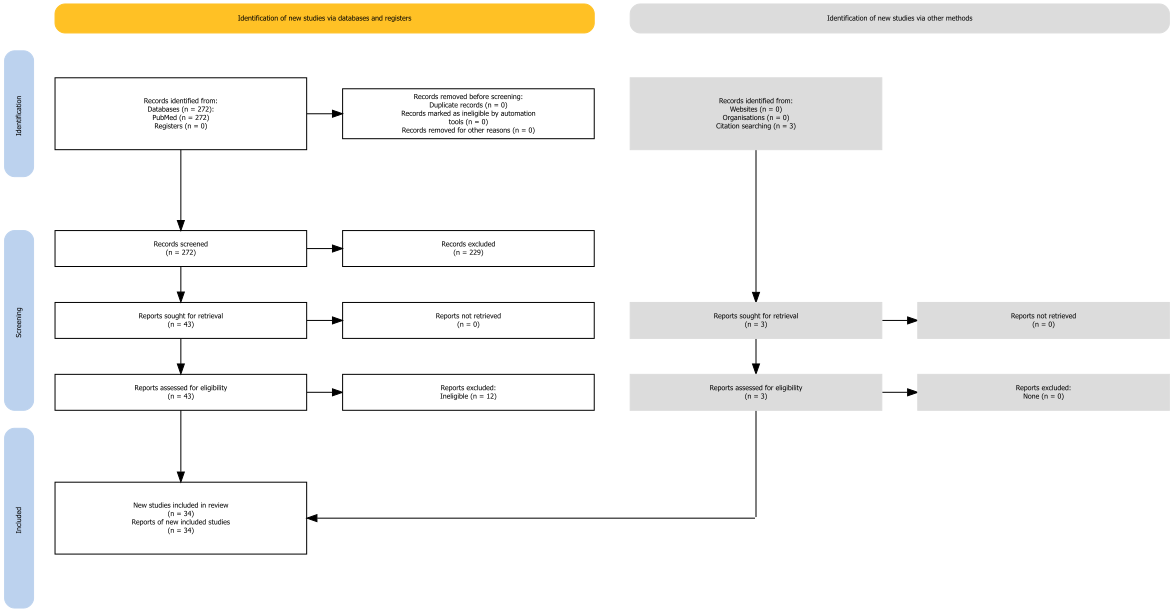
\includegraphics[width=\textwidth]{prisma_flow.png}
\caption{PRISMA 2020 source selection flow.}
\label{fig:prisma}
\end{figure}


The flow diagram shows a large reduction during title/abstract screening, with 229 records excluded before full-text assessment. The final corpus combines the 31 full-text inclusions with three citation-backtracked papers, which is important because the backtracked studies contributed directly to the final map rather than serving only as contextual references.

\subsection{Study and Participant Characteristics}
\begin{table}[H]
\centering
\caption{Baseline study and participant characteristics from \texttt{tables/table1.csv}.}
\label{tab:baseline-characteristics}
\small
\begin{tabularx}{\textwidth}{@{}p{0.34\textwidth}X p{0.24\textwidth}@{}}
\toprule
Characteristic & Summary & Denominator / missing data \\
\midrule
Included studies & 34 studies & 34/34 reported \\
Aggregate sample size & 1,593 participants & Reported in 30/34 studies; 4 unreported \\
Study sample size & Mean $\pm$ SD: 53.1 $\pm$ 97.9; Median [IQR]: 29.0 [19.3--46.8] & Calculated among 30 studies reporting \texttt{N\_Total} \\
Study mean age & Mean $\pm$ SD: 22.3 $\pm$ 6.1 years; Median [IQR]: 21.3 [19.8--23.7] & Calculated among 26 studies reporting \texttt{Age\_Mean}; 8 unreported \\
Estimated sex distribution & Male: 827.0 (53.5\%); Female: 720.0 (46.5\%) & Estimated among 1,547 participants from 29 studies reporting both sample size and male percentage; 5 studies lacked sufficient data \\
\addlinespace
Athlete level & Competitive: 14 (41.2\%); Recreational: 12 (35.3\%); Elite: 8 (23.5\%) & 34/34 studies classified \\
Study design & Experimental other: 19 (55.9\%); Experimental RCT: 9 (26.5\%); Observational cross-sectional: 3 (8.8\%); Experimental before-after: 2 (5.9\%); Observational retrospective: 1 (2.9\%) & 34/34 studies classified \\
Sport discipline & Not sport-specific/none: 7 (20.6\%); Various: 5 (14.7\%); Running: 4 (11.8\%); Swimming: 3 (8.8\%); Freediving: 3 (8.8\%); Resistance training: 2 (5.9\%); single-study disciplines: 10 (29.4\%) & 34/34 studies classified \\
\addlinespace
Race or ethnicity reporting & Reported: 0 (0.0\%); Not reported: 34 (100.0\%) & 34/34 studies assessed \\
Baseline anthropometrics reported & Reported: 23 (67.6\%); Not reported: 11 (32.4\%) & 34/34 studies assessed \\
Attrition noted & Yes: 8 (23.5\%); No: 26 (76.5\%) & 34/34 studies assessed \\
\bottomrule
\end{tabularx}
\end{table}


Table~\ref{tab:baseline-characteristics} shows that the mapped evidence base primarily reflects young adult cohorts, with sample-size information available for most studies and an aggregate extractable sample exceeding 1,500 participants. The participant pool was modestly male-predominant among studies with extractable sex data, and the cohort base was mainly competitive or recreational rather than exclusively elite. Missing age, sex, race/ethnicity, anthropometric, and attrition information remained common enough to limit denominator certainty and external-validity judgments.

\begin{table}[tbp]
\centering
\caption{Summary of the mapped evidence base.}
\label{tab:evidence-map}
\begin{tabularx}{\textwidth}{@{}lX@{}}
\toprule
Domain & Finding \\
\midrule
Initial PubMed records & 272 \\
Title/abstract retained & 43 \\
Full-text retained & 31 \\
Citation-backtracked additions & 3 \\
Included sources in extraction dataset & 34 \\
Publication years represented & 2004--2026 in cleaned extraction; one source has a 2000 bibliography year \\
Experimental studies & 31/34 (91.2\%) \\
Observational studies & 2/34 (5.9\%) \\
Unclear design classification & 1/34 (2.9\%) \\
Studies with age data & 26 studies, 1185 participants \\
Weighted mean age & 26.7 years (pooled SD 10.2) \\
Studies with sex data & 1234 participants; estimated male proportion 51.5\% \\
\bottomrule
\end{tabularx}
\end{table}

\begin{table}[tbp]
\centering
\caption{Breathing-training categories in the extracted intervention records.}
\label{tab:bt-categories}
\begin{tabular}{@{}lrr@{}}
\toprule
Category & Records & Percentage \\
\midrule
Other or unclear & 11 & 31.4\% \\
Hyperventilation & 9 & 25.7\% \\
Paced breathing & 9 & 25.7\% \\
Hypoventilation & 3 & 8.6\% \\
Pranayama/yogic breathing & 2 & 5.7\% \\
Breath holding/Valsalva & 1 & 2.9\% \\
\bottomrule
\end{tabular}
\end{table}

\begin{table}[tbp]
\centering
\caption{Most represented sport contexts.}
\label{tab:sports}
\begin{tabular}{@{}lrr@{}}
\toprule
Sport context & Studies & Percentage \\
\midrule
Not sport-specific & 7 & 20.6\% \\
Various/mixed sports & 6 & 17.6\% \\
Freediving & 3 & 8.8\% \\
Running & 3 & 8.8\% \\
Swimming & 3 & 8.8\% \\
Resistance training & 2 & 5.9\% \\
Single-study contexts & 10 & 29.4\% \\
\bottomrule
\end{tabular}
\end{table}

\begin{table}[tbp]
\centering
\caption{Exploratory random-effects syntheses from comparable outcome clusters.}
\label{tab:meta}
\begin{tabular}{@{}lrrrrr@{}}
\toprule
Cluster & $k$ & Pooled $g$ & 95\% CI & $p$ & $I^2$ \\
\midrule
Hyperventilation and power outcomes & 6 & 0.30 & -0.00 to 0.60 & 0.052 & 0.0\% \\
Paced breathing and reaction outcomes & 4 & -0.15 & -0.45 to 0.15 & 0.335 & 57.9\% \\
Hypoventilation and repeated-sprint outcomes & 1 & -- & Not pooled & -- & -- \\
\bottomrule
\end{tabular}

\vspace{1mm}
\parbox{0.92\textwidth}{\footnotesize Positive values were coded as favoring the breathing intervention after direction normalization. These syntheses are exploratory because outcome clusters were small and heterogeneous.}
\end{table}

\begin{table}[tbp]
\centering
\caption{Feasibility and safety reporting.}
\label{tab:feasibility}
\begin{tabularx}{\textwidth}{@{}lX@{}}
\toprule
Item & Extracted finding \\
\midrule
Studies with parseable adherence data & 0 \\
Studies with parseable dropout data & 0 \\
Adverse event mentions & Dizziness, heaviness, numbness, tingling, and pulmonary edema \\
Main safety pattern & Hyperventilation-related sensory symptoms were reported in one source; pulmonary edema was noted in a freediving/hook-breathing context \\
\bottomrule
\end{tabularx}
\end{table}


\subsection{Characteristics of included sources}
The cleaned dataset mapped 34 sources spanning 2004--2026, with one bibliographic discrepancy in which the extraction identifier `Durand2004' corresponds to a 2000 BibTeX record. Most studies were experimental (31/34, 91.2\%), while two were observational and one remained unclear. However, only eight records were classified as parallel or controlled trials; most were crossover, repeated-measures, acute, pilot, or otherwise categorized as experimental-other.

Across studies with age data, 1185 participants contributed to a weighted mean age of 26.7 years. Sex data were available for 1234 participants and suggested an approximately balanced overall sample, with an estimated male proportion of 51.5\%. Sport contexts were dispersed. The most frequent categories were not sport-specific, mixed/various sports, freediving, running, and swimming, while many sport contexts appeared only once.

\begin{landscape}
\begin{longtable}{@{}p{0.17\linewidth}p{0.10\linewidth}p{0.20\linewidth}p{0.15\linewidth}p{0.16\linewidth}p{0.12\linewidth}@{}}
\caption{Characteristics of included sources.}
\label{tab:study-characteristics}\\
\toprule
Study ID & Year & Design & Sport/context & Level/population & Breathing category \\
\midrule
\endfirsthead
\toprule
Study ID & Year & Design & Sport/context & Level/population & Breathing category \\
\midrule
\endhead
\bottomrule
\endfoot
Durand2004 & 2004 & Observational cross-sectional & Endurance & Competitive & Other/unclear \\
Spiering2004 & 2004 & Experimental, other & Various & Competitive & Other/unclear \\
Lindholm2005 & 2005 & Experimental, other & Freediving & Elite & Other/unclear \\
Malakhov2014 & 2014 & Experimental, other & Various & Competitive & Hyperventilation \\
Sakamoto2014 & 2014 & Experimental, other & Various & Competitive & Hyperventilation \\
Sakamoto2015 & 2015 & Experimental, other & Various & Competitive & Hyperventilation \\
Stavrou2015 & 2015 & Experimental RCT & Swimming & Competitive & Hypoventilation \\
Hakked2017 & 2017 & Experimental RCT & Swimming & Competitive & Pranayama/yogic \\
Sakamoto2018 & 2018 & Experimental, other & Various & Competitive & Hyperventilation \\
Fernandez2019 & 2019 & Experimental, other & Freediving & Elite & Other/unclear \\
Citherlet2021 & 2021 & Experimental, other & Running & Recreational & Hyperventilation; Wim Hof \\
Taylor2021 & 2021 & Experimental, other & Not sport-specific & Recreational & Paced breathing \\
Vaidya2021 & 2021 & Experimental, other & Cricket & Competitive & Pranayama/yogic \\
Bahensky2021 & 2021 & Experimental RCT & Running & Competitive & Pranayama/yogic \\
Marko2022 & 2022 & Experimental RCT & Running & Elite & Hyperventilation; Wim Hof \\
You2023 & 2023 & Experimental, other & Not sport-specific & Recreational & Paced breathing \\
Braham2024 & 2024 & Experimental RCT & Soccer & Competitive & Hypoventilation \\
Li2024 & 2024 & Experimental, other & Not sport-specific & Recreational & Paced breathing \\
Merlin2024 & 2024 & Experimental RCT & Swimming & Elite & Paced breathing \\
Sikora2024 & 2024 & Observational cross-sectional & Various & Competitive & Other/unclear \\
Woorons2024 & 2024 & Experimental RCT & Judo & Elite & Hypoventilation \\
Deniz2025 & 2025 & Experimental, other & Resistance training & Recreational & Breath holding; Valsalva \\
Fernandez2025 & 2025 & Experimental, other & Freediving & Elite & Other/unclear \\
Fesseler2025 & 2025 & Experimental, other & Running & Recreational & Hyperventilation \\
Fox2025 & 2025 & Experimental RCT & Not sport-specific & Recreational & Hyperventilation; Wim Hof \\
Kasap2025 & 2025 & Experimental, other & Cycling & Recreational & Paced breathing \\
Yilmaz2025 & 2025 & Experimental, other & Team sports & Competitive & Hyperventilation \\
Chiron2026 & 2026 & Experimental RCT & Track and field & Elite & Paced breathing \\
Devipriya2026 & 2026 & Experimental before-after & Not sport-specific & Recreational & Pranayama/yogic \\
FernandezBarradas2026 & 2026 & Experimental before-after & American football & Competitive & Paced breathing \\
Iskra2026 & 2026 & Experimental, other & Not sport-specific & Recreational & Paced breathing \\
Katz2026 & 2026 & Experimental, other & Resistance training & Recreational & Other/unclear \\
Raidl2026 & 2026 & Experimental, other & Not sport-specific & Recreational & Paced breathing \\
Tomita2026 & 2026 & Experimental, other & Skating & Competitive & Paced breathing \\
\end{longtable}
\end{landscape}


\begin{figure}[H]
\centering
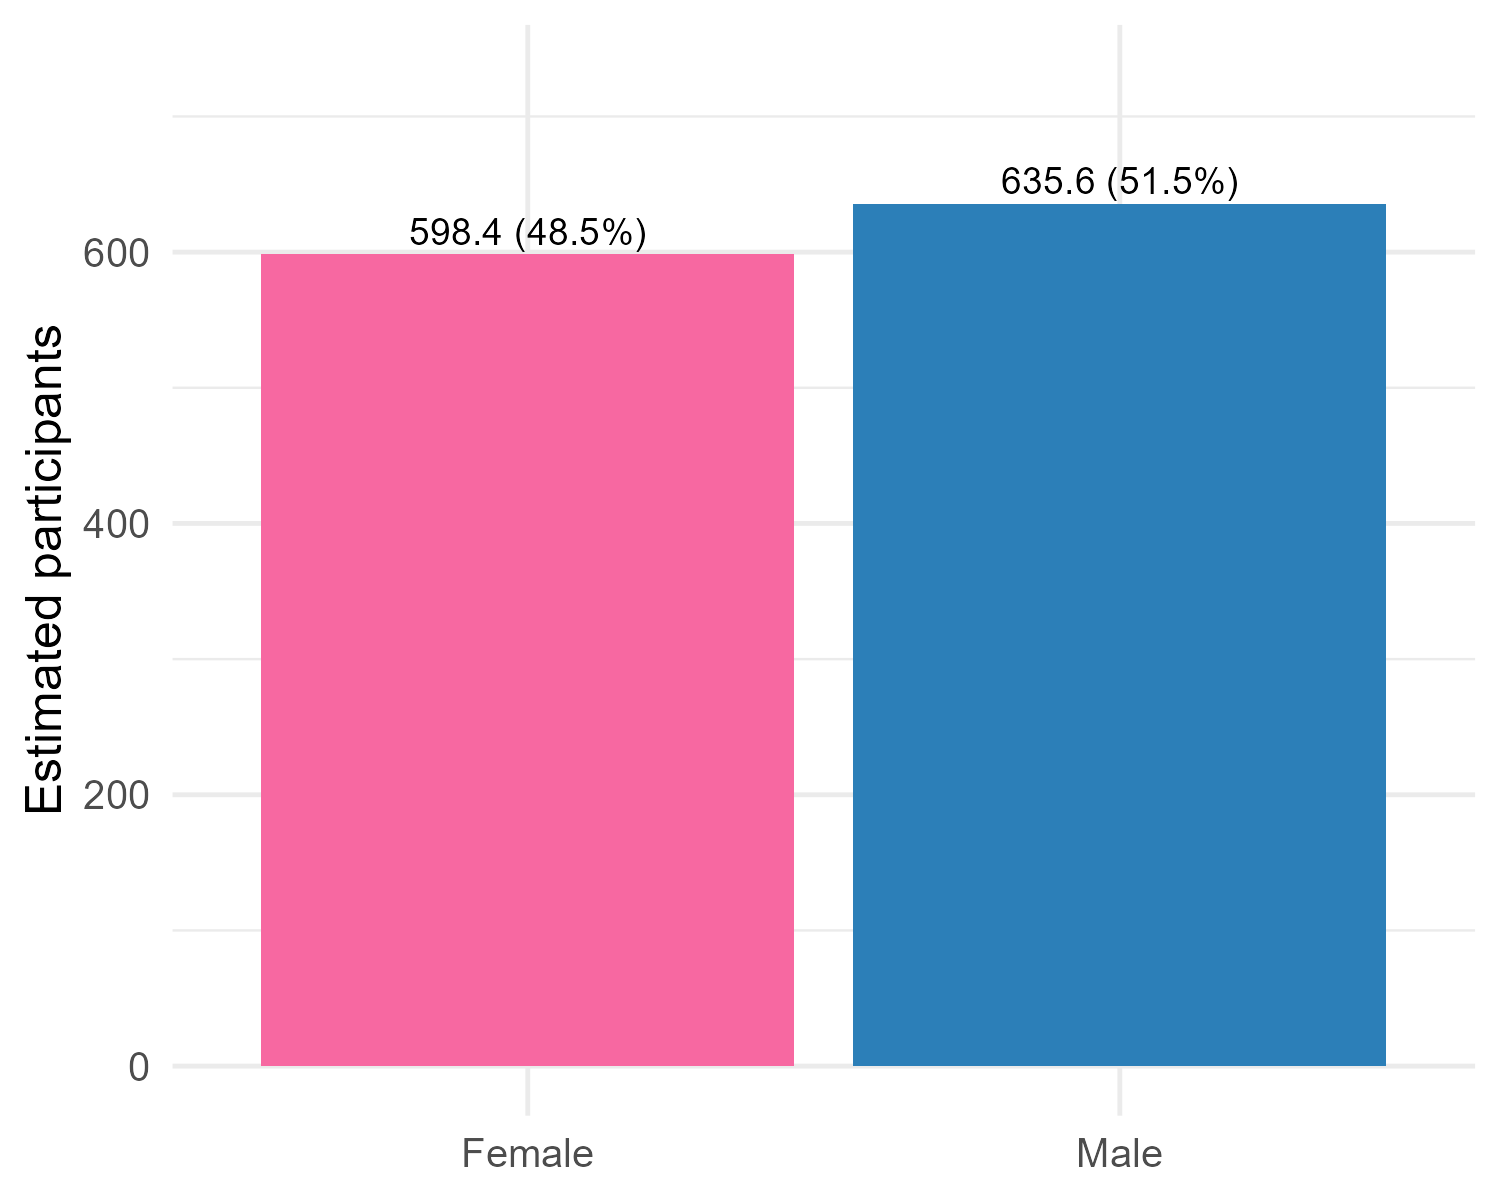
\includegraphics[width=0.78\textwidth]{sex_distribution.png}
\caption{Estimated sex distribution in studies with extractable sex data.}
\label{fig:sex-distribution}
\end{figure}

The sex-distribution plot indicates that the extractable participant pool was approximately balanced overall, but this aggregate masks study-level imbalances. Several sport-specific subfields, such as freediving, resistance training, and some team-sport contexts, were male-dominant in the extraction, while other studies contained mixed or female samples. This limits certainty about whether effects generalize equally across sex and sport contexts.

\subsection{Publication trends}
\begin{figure}[H]
\centering

\includegraphics[width=0.90\textwidth]{publication_trend.png}
\caption{Annual publication counts and fitted exploratory trend lines.}
\label{fig:publication-trend}
\end{figure}

Publication volume increased most clearly in the recent extraction years, with the highest annual counts in 2025 and 2026. This pattern suggests growing interest in non-device breathing techniques for sport and performance, although the apparent acceleration should be interpreted cautiously because 2026 records may represent early online publications and because the search was conducted on 15 June 2025 with subsequent project extraction updates.

\subsection{Study design and sport context}
\begin{figure}[H]
\centering
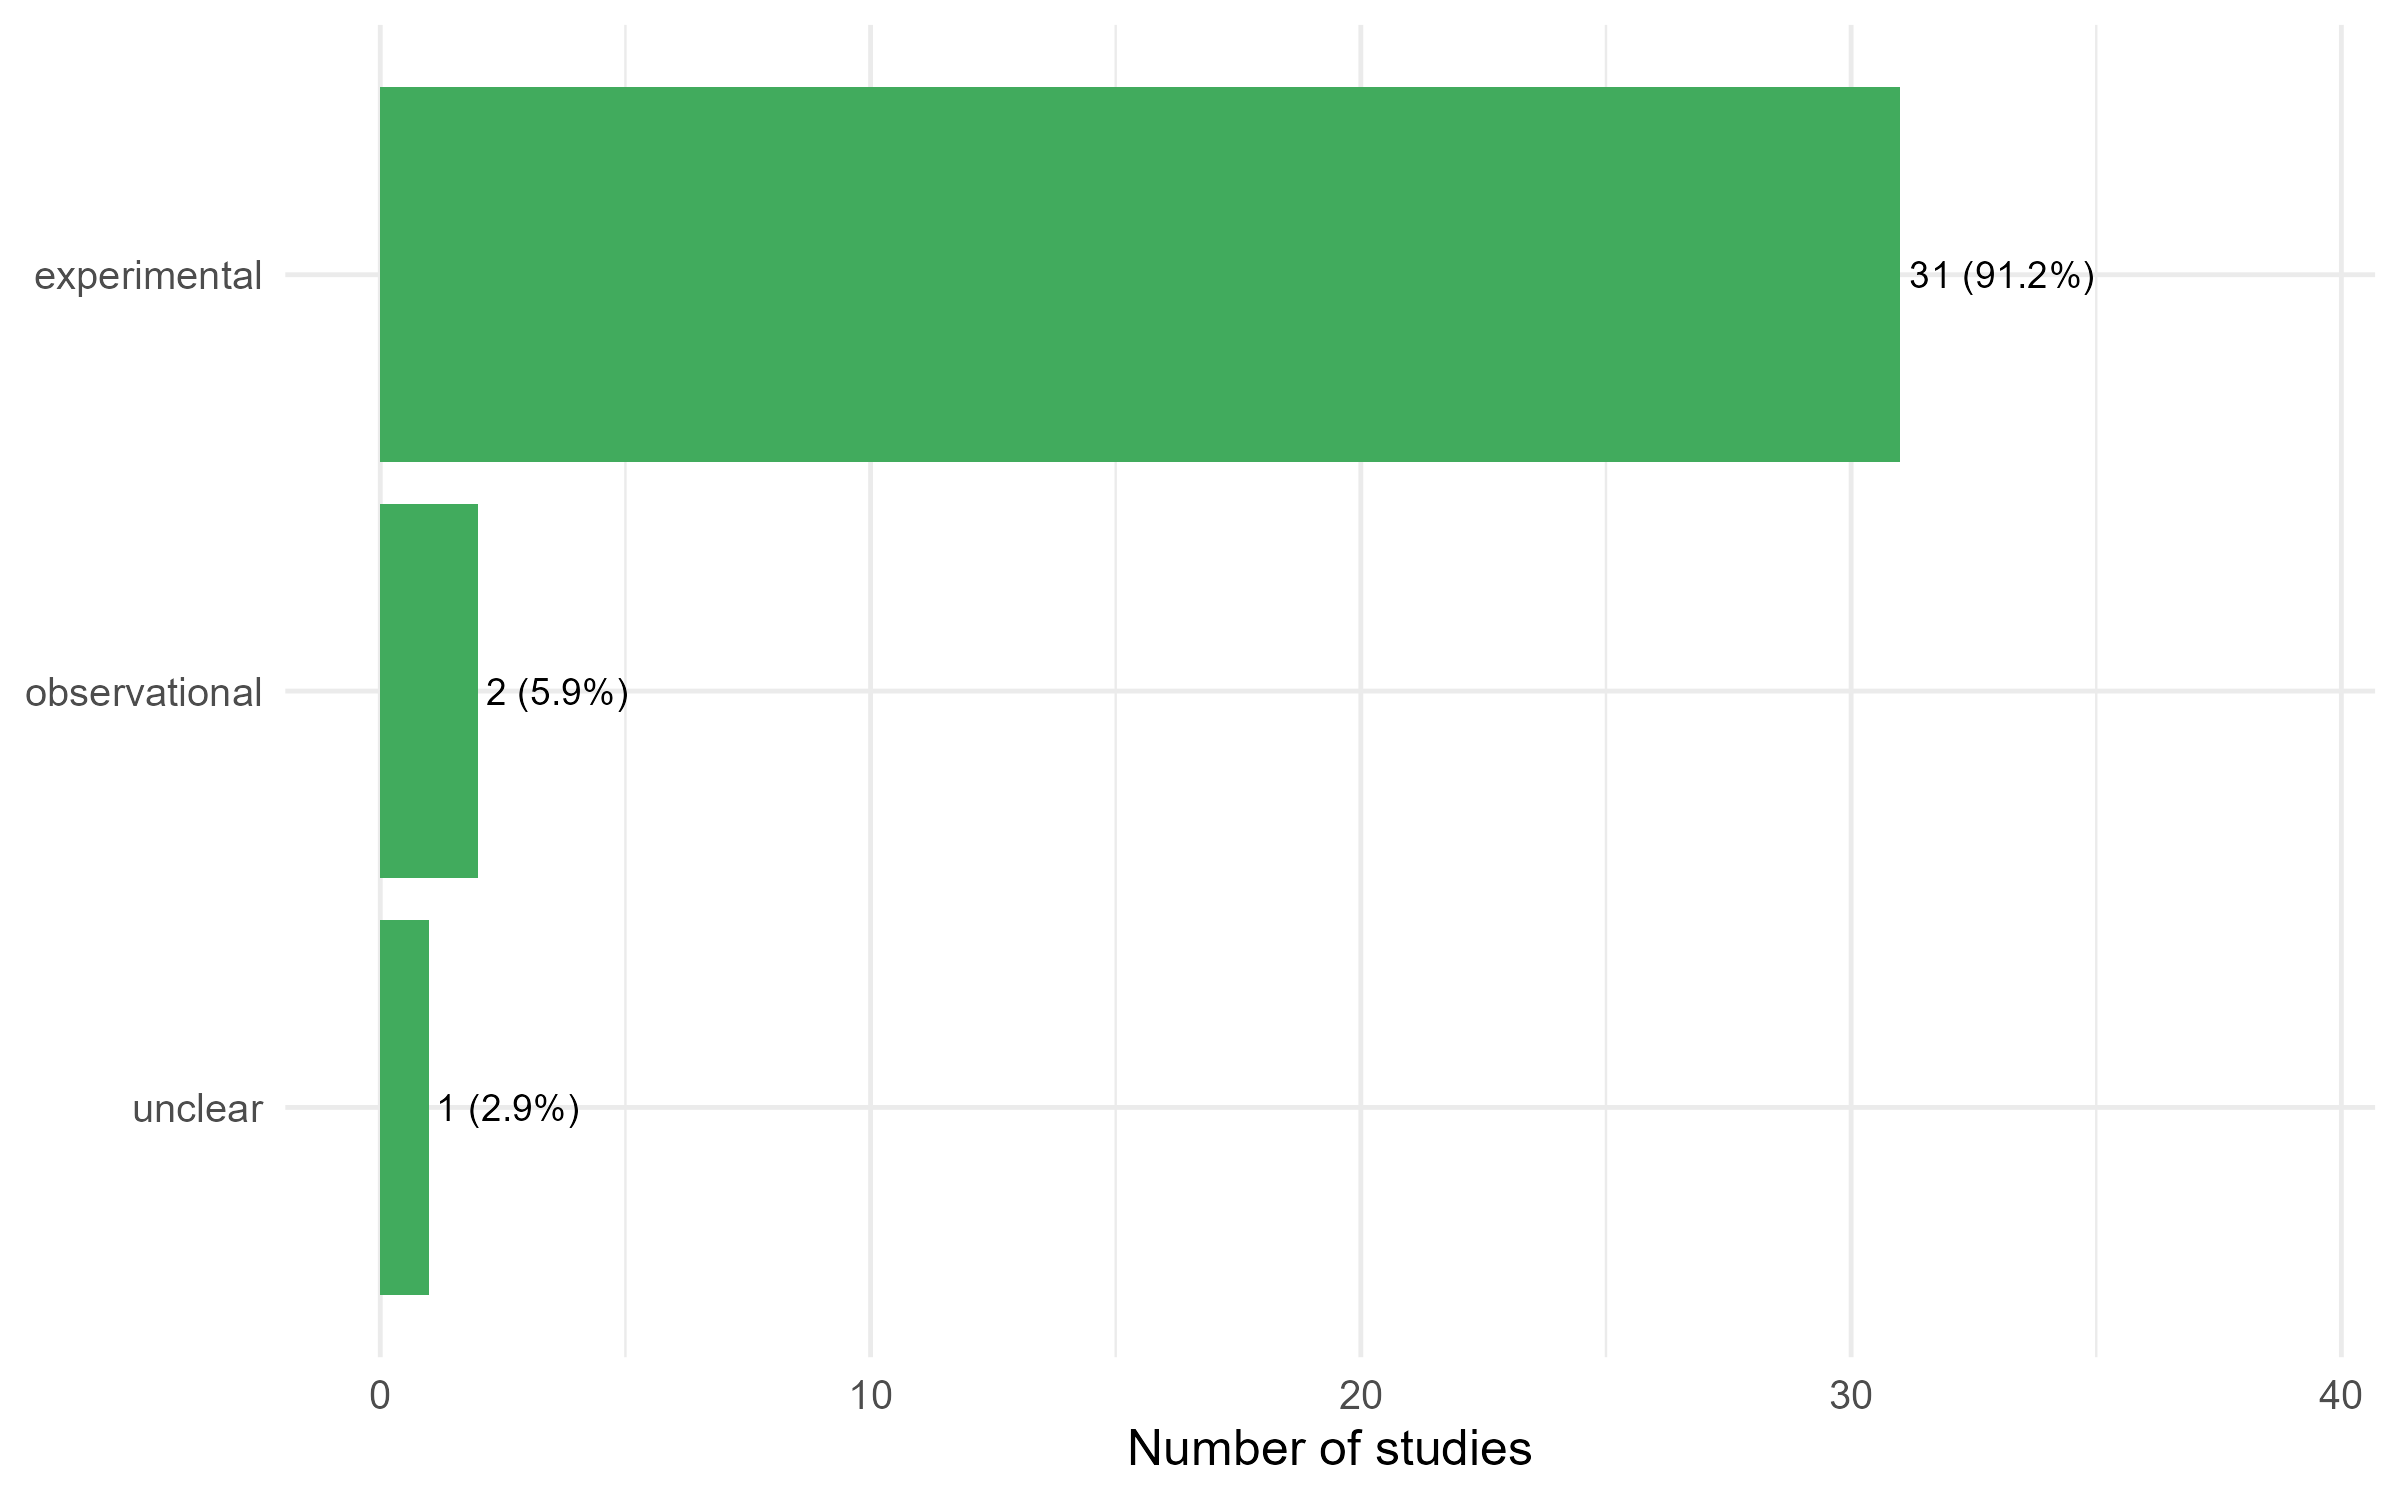
\includegraphics[width=0.78\textwidth]{study_design_broad_distribution.png}
\caption{Broad study-design distribution.}
\label{fig:design-broad}
\end{figure}

The broad design distribution shows that the evidence base is dominated by experimental studies. This is encouraging for intervention mapping, but the category is broad and includes acute crossover, repeated-measures, pilot, and before-after designs as well as randomized controlled trials.

\begin{figure}[H]
\centering
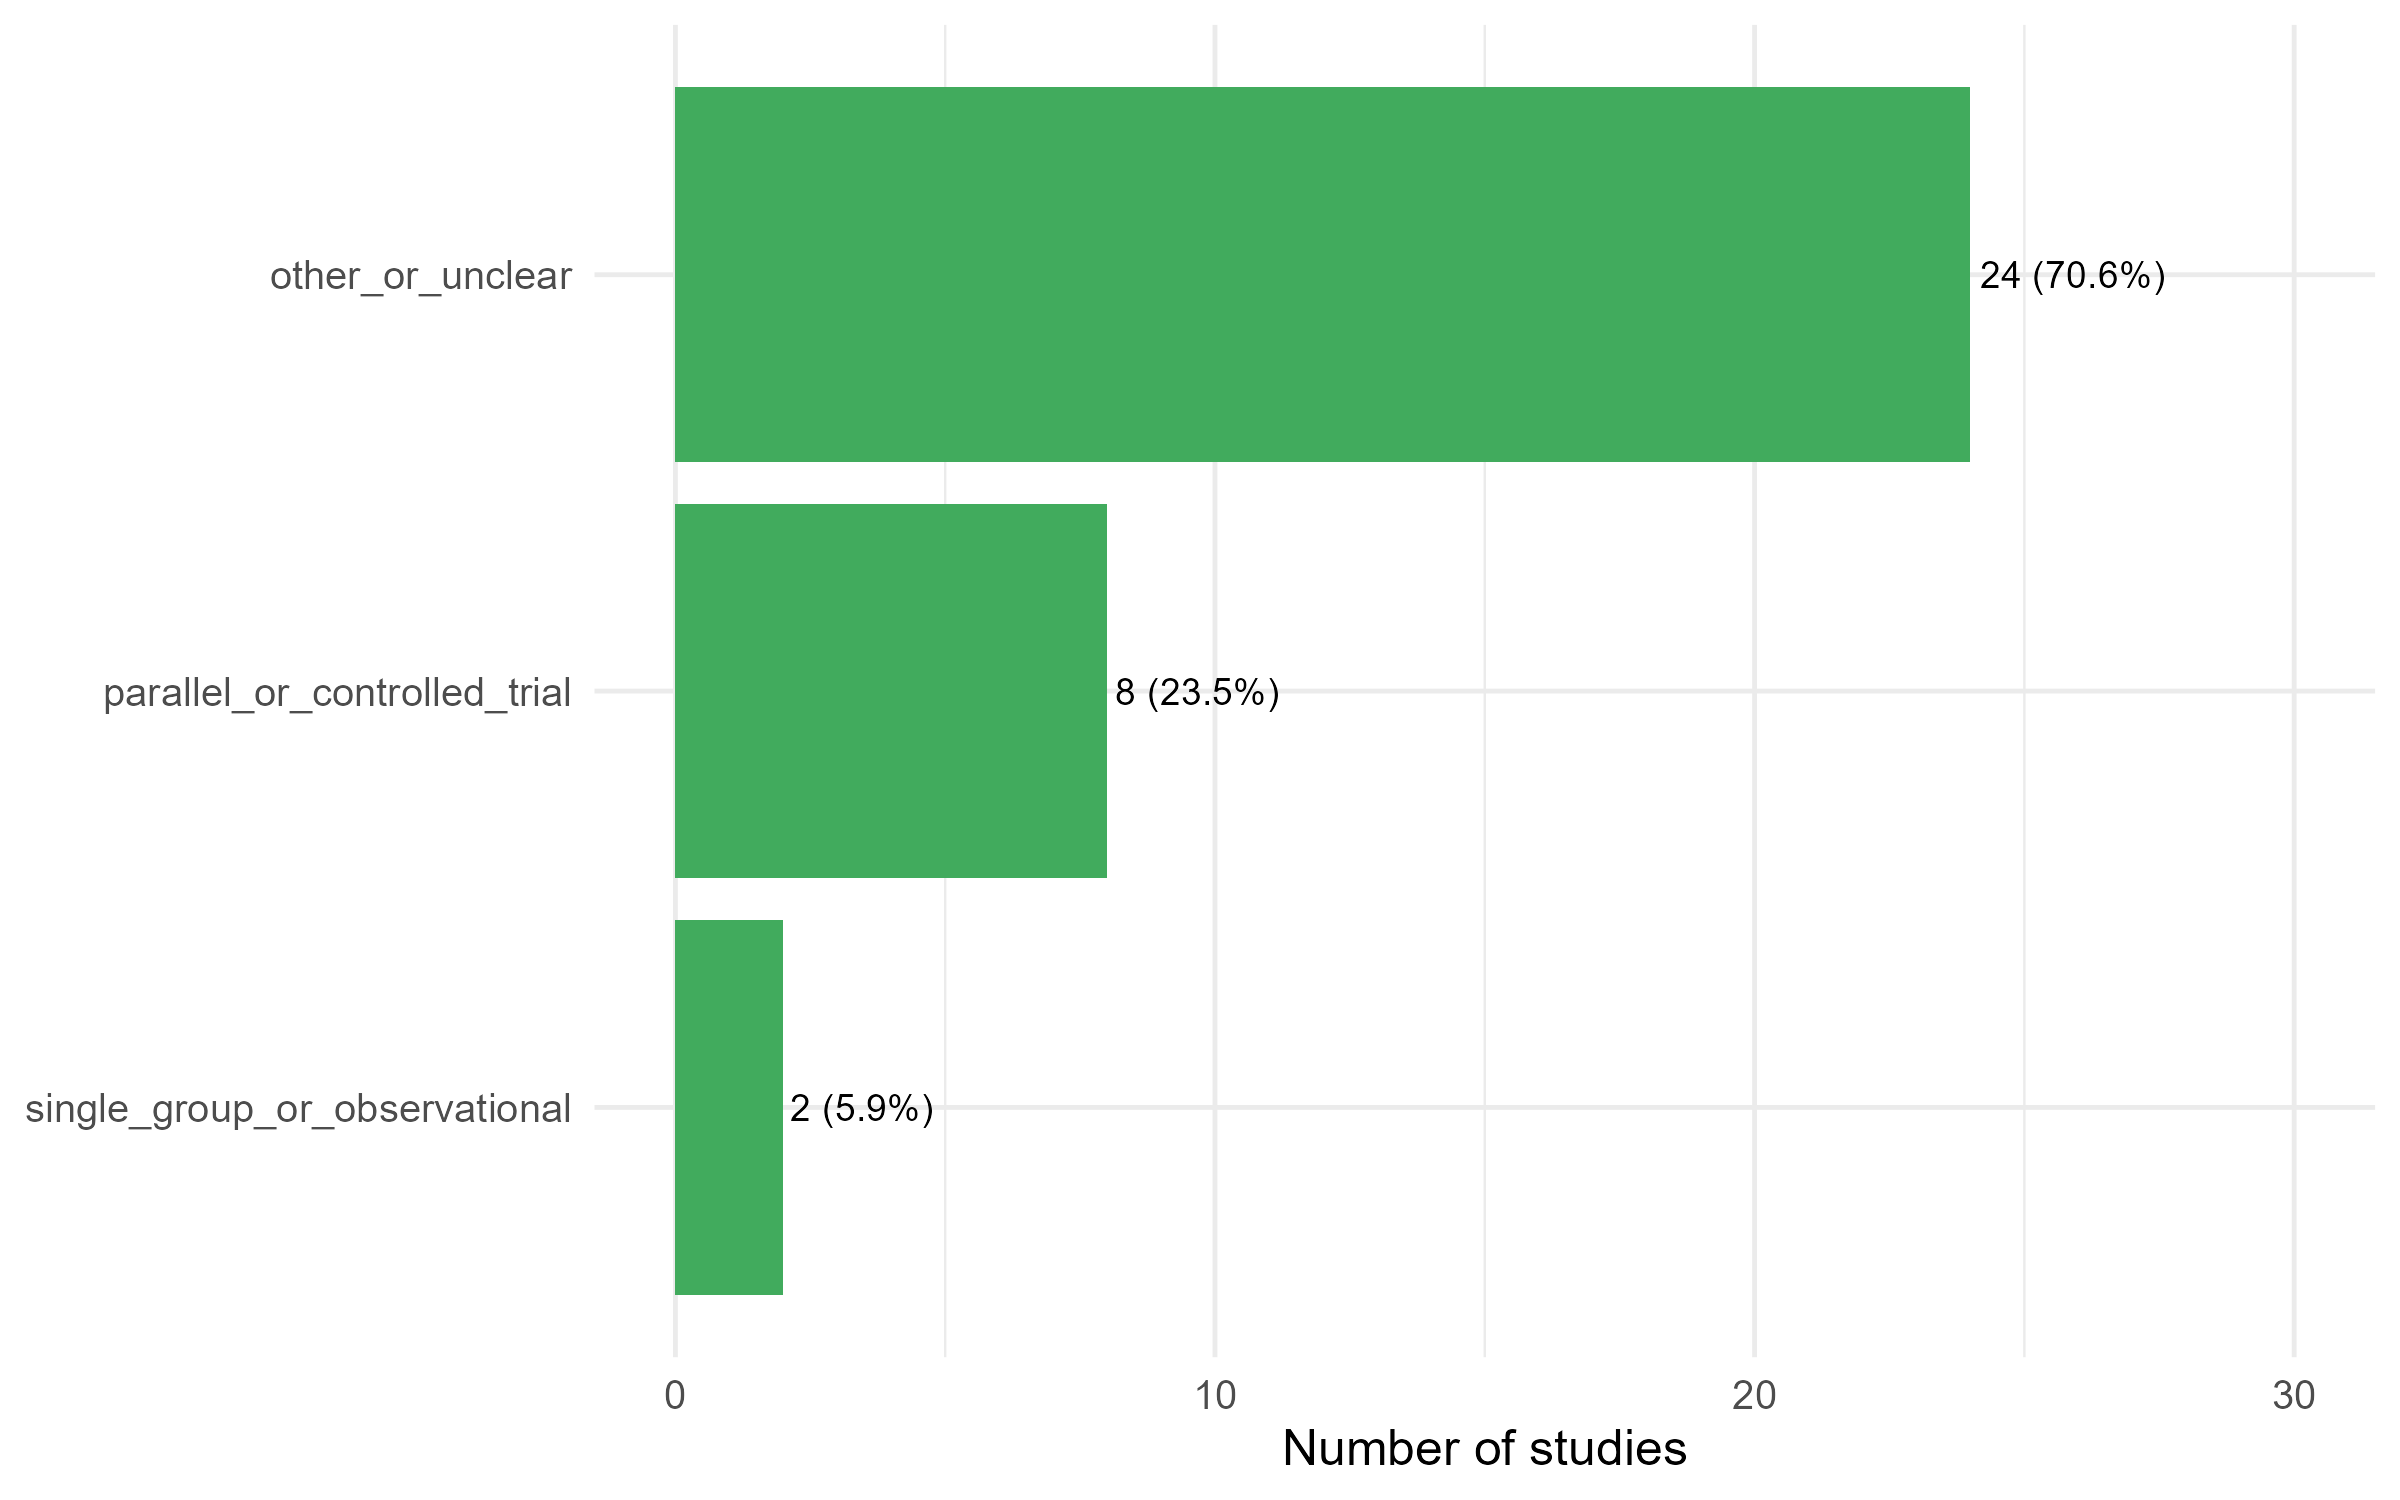
\includegraphics[width=0.78\textwidth]{study_design_distribution.png}
\caption{Detailed study-design distribution after cleaning.}
\label{fig:design-detailed}
\end{figure}

The detailed design plot clarifies that most records were categorized as other or unclear experimental designs, while parallel or controlled trials represented a smaller portion of the map. This supports the main methodological conclusion: the literature is active, but many studies are not yet designed or reported in a way that supports strong causal or sport-practice recommendations.

\begin{figure}[H]
\centering
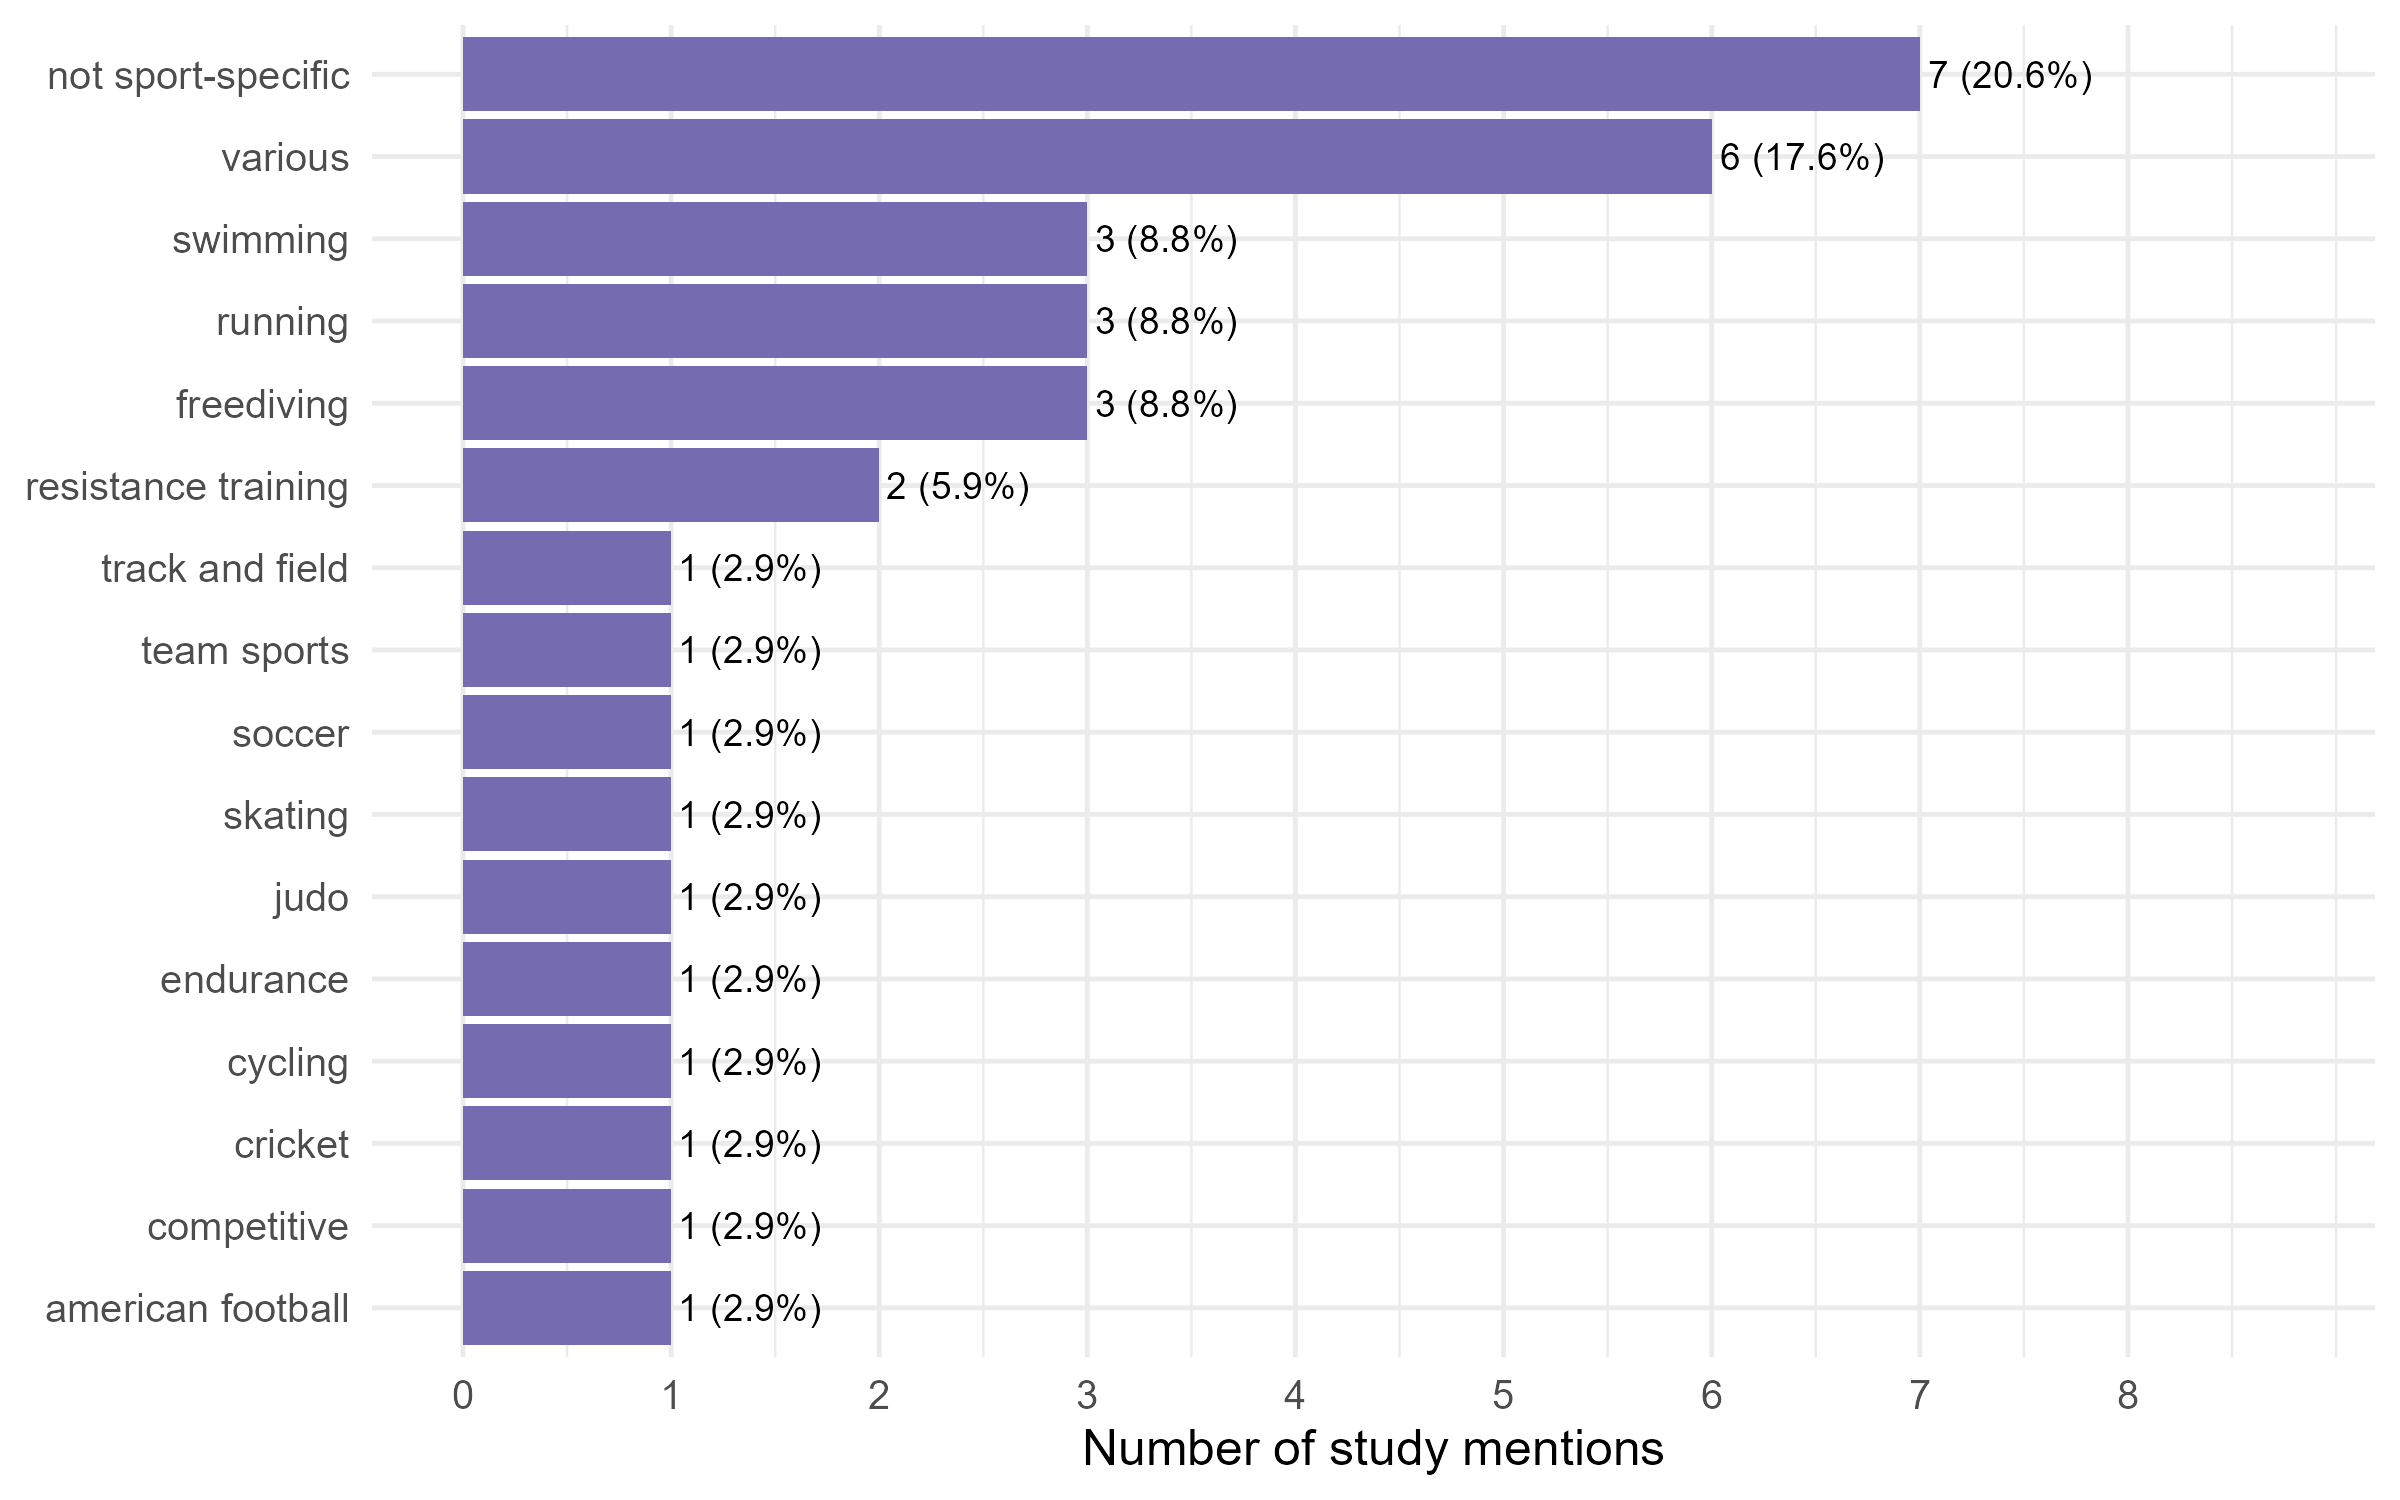
\includegraphics[width=0.92\textwidth]{sport_distribution.png}
\caption{Distribution of sport and performance contexts.}
\label{fig:sport-distribution}
\end{figure}

Sport context was widely dispersed. Not sport-specific and mixed-sport studies formed the largest groups, followed by freediving, running, and swimming. The long tail of single-study sport contexts means that many practical sport-specific questions cannot yet be answered from replicated evidence.

\subsection{Breathing-intervention categories and dose}
The most frequent extracted categories were other/unclear breathing strategies, hyperventilation, and paced breathing. Hypoventilation, pranayama/yogic breathing, and breath holding or Valsalva-type strategies were less common. Dose reporting was uneven. Among parseable records, the median frequency was one session per week, and the median duration was one day, indicating that much of the literature concerns acute or short exposure protocols rather than extended training programs.

\begin{figure}[H]
\centering
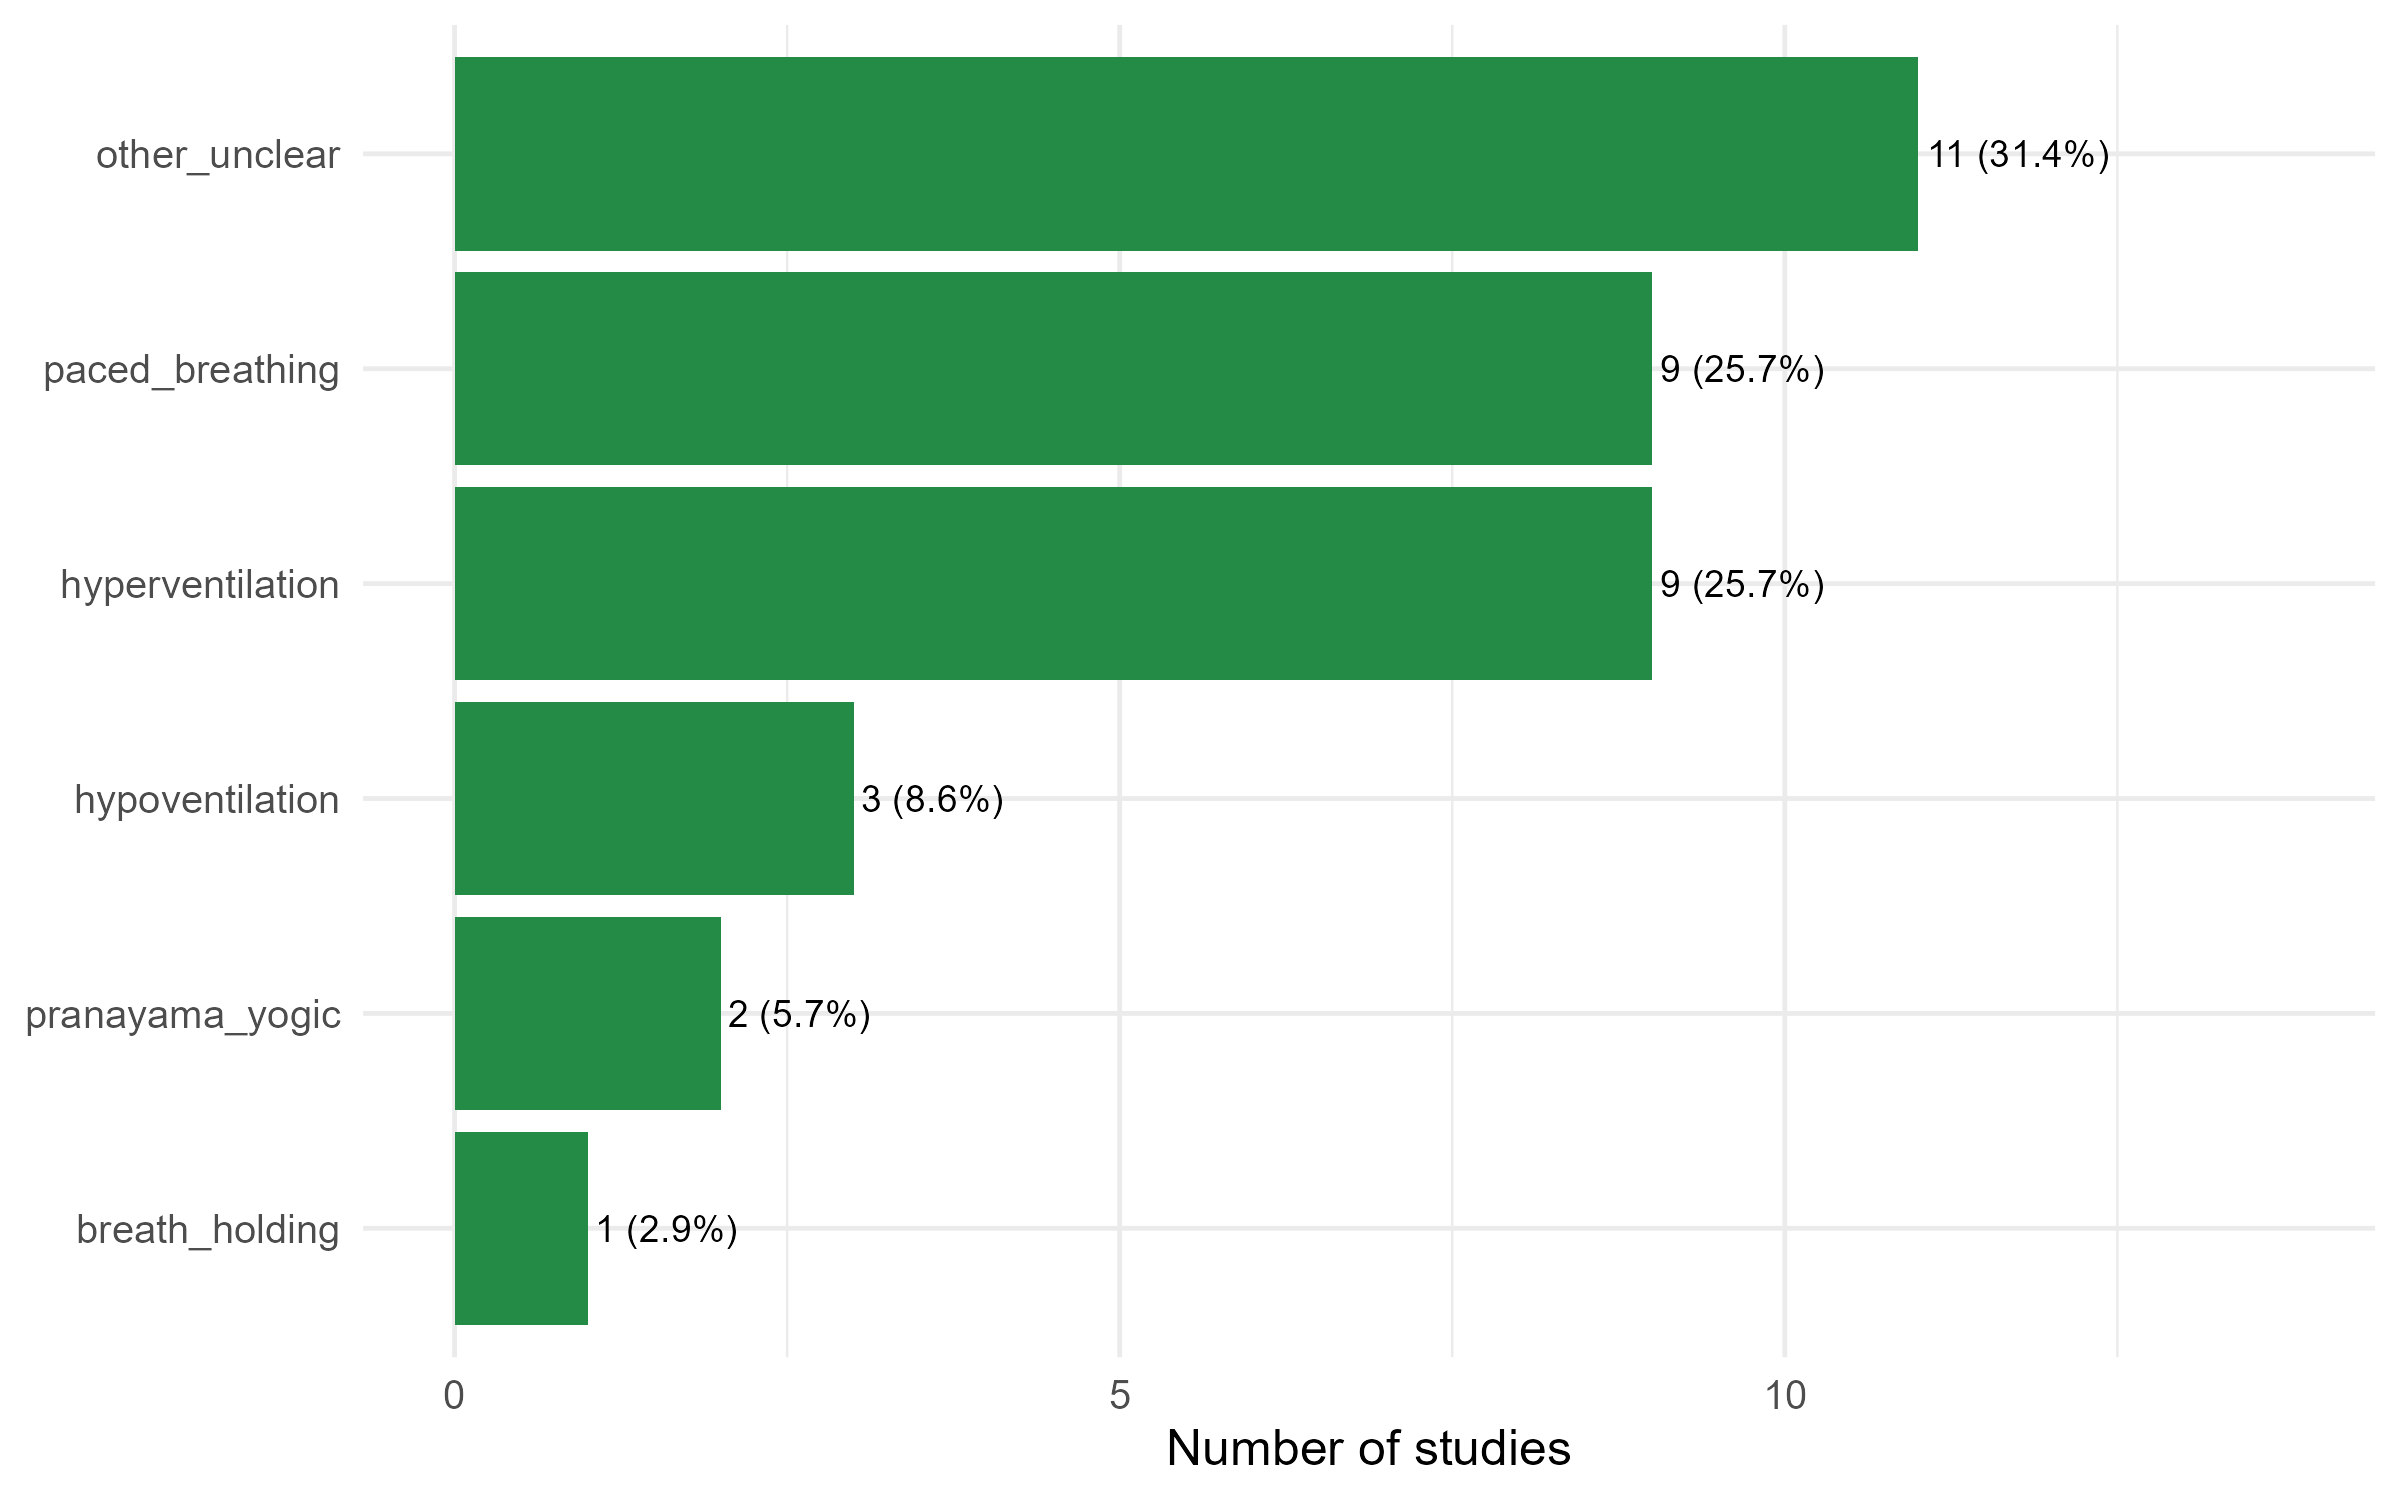
\includegraphics[width=0.82\textwidth]{bt_category_distribution.png}
\caption{Distribution of breathing-training categories in the cleaned extraction.}
\label{fig:bt-category}
\end{figure}

The breathing-category plot shows that the literature is not organized around one dominant intervention. Hyperventilation and paced breathing were equally represented among classified categories, whereas hypoventilation, pranayama/yogic breathing, and breath holding were less frequent. The large other/unclear category reflects both genuinely mixed interventions and inconsistent reporting terminology.

\begin{figure}[H]
\centering

\includegraphics[width=0.82\textwidth]{intervention_duration_distribution.png}
\caption{Distribution of intervention duration among parseable records.}
\label{fig:duration}
\end{figure}

The duration plot reinforces that the mapped evidence is heavily weighted toward acute or very short protocols. A smaller subset used multi-week interventions, which makes it difficult to separate immediate psychophysiological effects from adaptations that require repeated training exposure.

\subsection{Outcome synthesis}
Outcome measures were highly heterogeneous, covering pulmonary function, blood gases, sprint and power outcomes, reaction and movement time, heart-rate variability, perceived exertion, anxiety, recovery states, oxygen saturation, and sport-specific performance. Because most outcome domains were represented by few studies, the scoping synthesis emphasizes mapping rather than definitive effect estimation.

Exploratory quantitative synthesis was possible for two outcome clusters. Hyperventilation-related power outcomes showed a small pooled effect favoring the intervention ($g=0.30$, 95\% CI -0.00 to 0.60, $p=0.052$, $I^2=0.0\%$). This estimate is compatible with a small beneficial effect but is borderline and should not be read as conclusive. Paced-breathing reaction outcomes were inconclusive ($g=-0.15$, 95\% CI -0.45 to 0.15, $p=0.335$, $I^2=57.9\%$). A hypoventilation repeated-sprint cluster had only one eligible effect and was not pooled.

\begin{figure}[H]
\centering
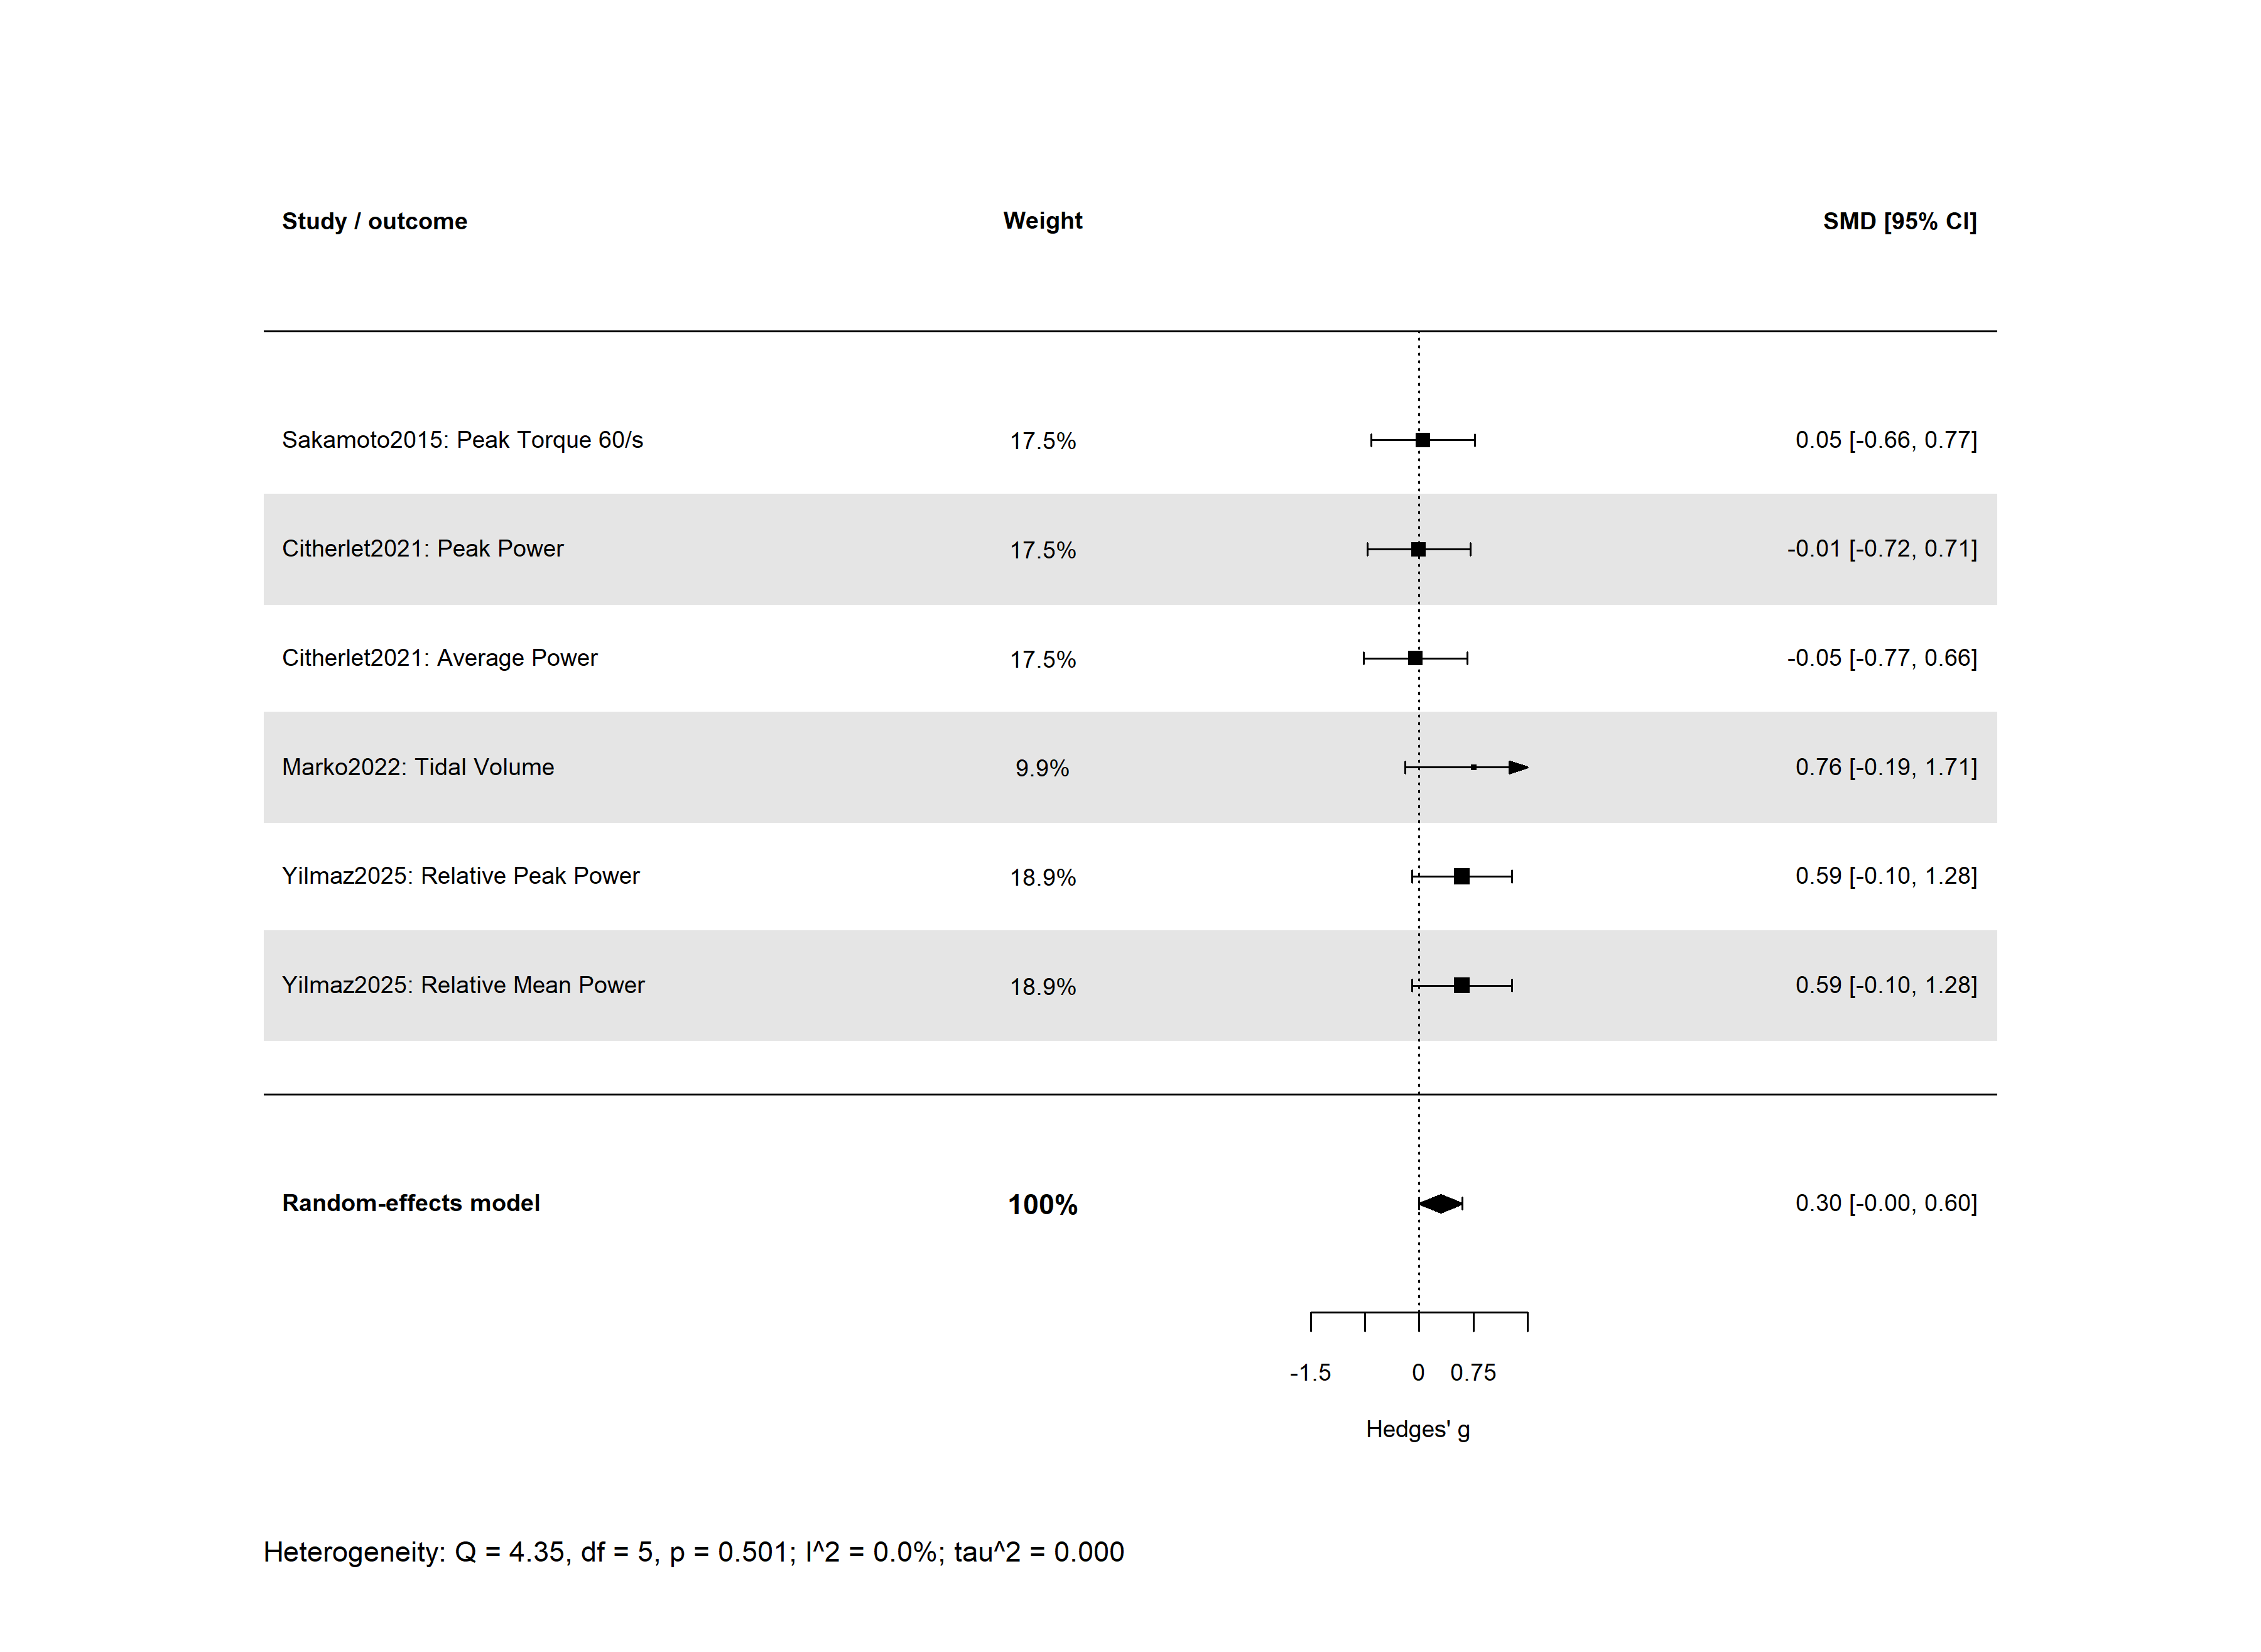
\includegraphics[width=0.92\textwidth]{forest_hyperventilation_power.png}
\caption{Exploratory forest plot for hyperventilation and power-related outcomes.}
\label{fig:forest-hyper}
\end{figure}

The hyperventilation forest plot shows a small pooled effect close to conventional statistical significance. Individual effects were not uniformly large, but the low estimated heterogeneity indicates that this may be one of the more coherent outcome clusters in the current map. Even so, the confidence interval touches the null, so the result should be treated as a hypothesis for targeted trials rather than proof of ergogenic benefit.

\begin{figure}[H]
\centering

\includegraphics[width=0.92\textwidth]{forest_paced_breathing_reaction.png}
\caption{Exploratory forest plot for paced breathing and reaction-related outcomes.}
\label{fig:forest-paced}
\end{figure}

The paced-breathing forest plot does not show a clear pooled benefit for reaction-related outcomes, and heterogeneity was moderate. This suggests that paced breathing may be context-dependent: effects may depend on whether the target is arousal control, recovery, anxiety, attentional readiness, or immediate motor response.

\subsection{Feasibility and safety}
Feasibility reporting was sparse. The cleaned outputs contained no parseable adherence summaries and no parseable dropout summaries. Adverse-event extraction identified sensory symptoms associated with hyperventilation, including dizziness, heaviness, numbness, and tingling, and pulmonary edema in a freediving/hook-breathing context. These findings do not establish incidence rates because reporting was incomplete and inconsistent, but they indicate that safety reporting should be mandatory in future studies of respiratory maneuvers that alter carbon dioxide, oxygen saturation, intrathoracic pressure, or autonomic state.

\begin{figure}[H]
\centering
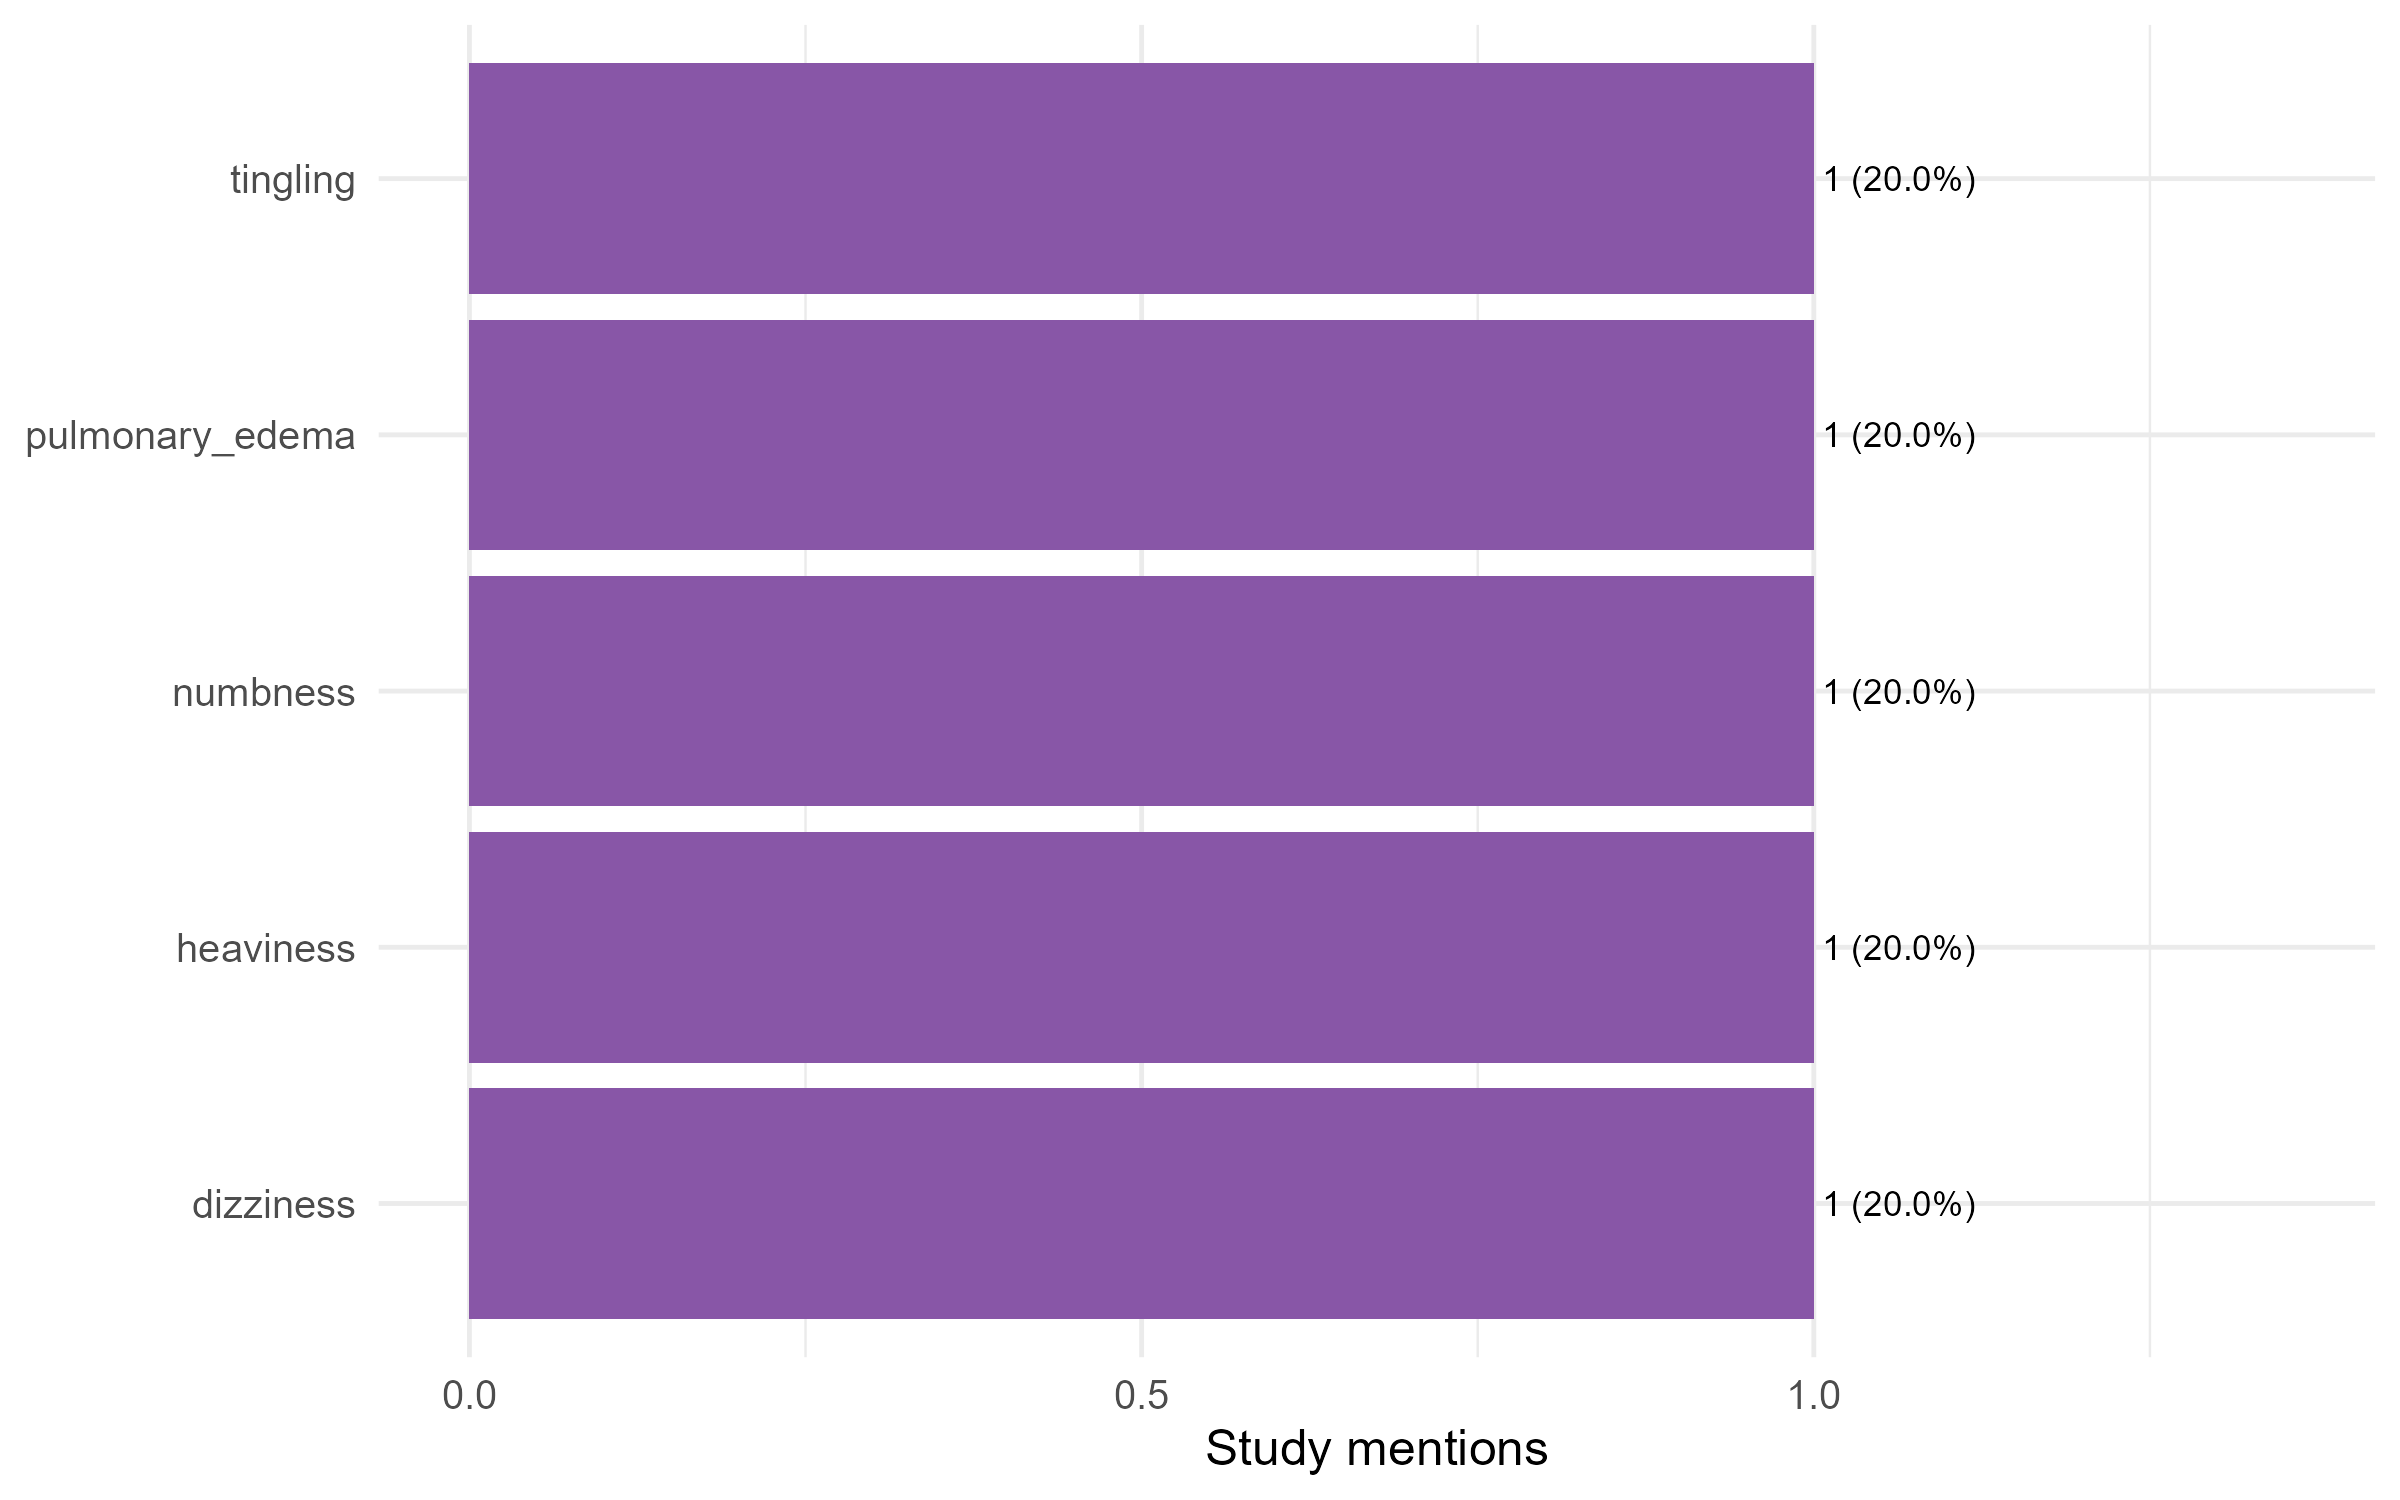
\includegraphics[width=0.82\textwidth]{adverse_events_by_bt.png}
\caption{Adverse-event mentions by breathing-technique category.}
\label{fig:adverse-events}
\end{figure}

The adverse-event plot shows few reported events, but the pattern is clinically relevant. Hyperventilation-related sensory symptoms are plausible consequences of hypocapnia and respiratory discomfort, while pulmonary edema in a freediving context points to a higher-risk domain where breathing maneuvers interact with pressure, hypoxia, and post-dive recovery.

\begin{figure}[H]
\centering
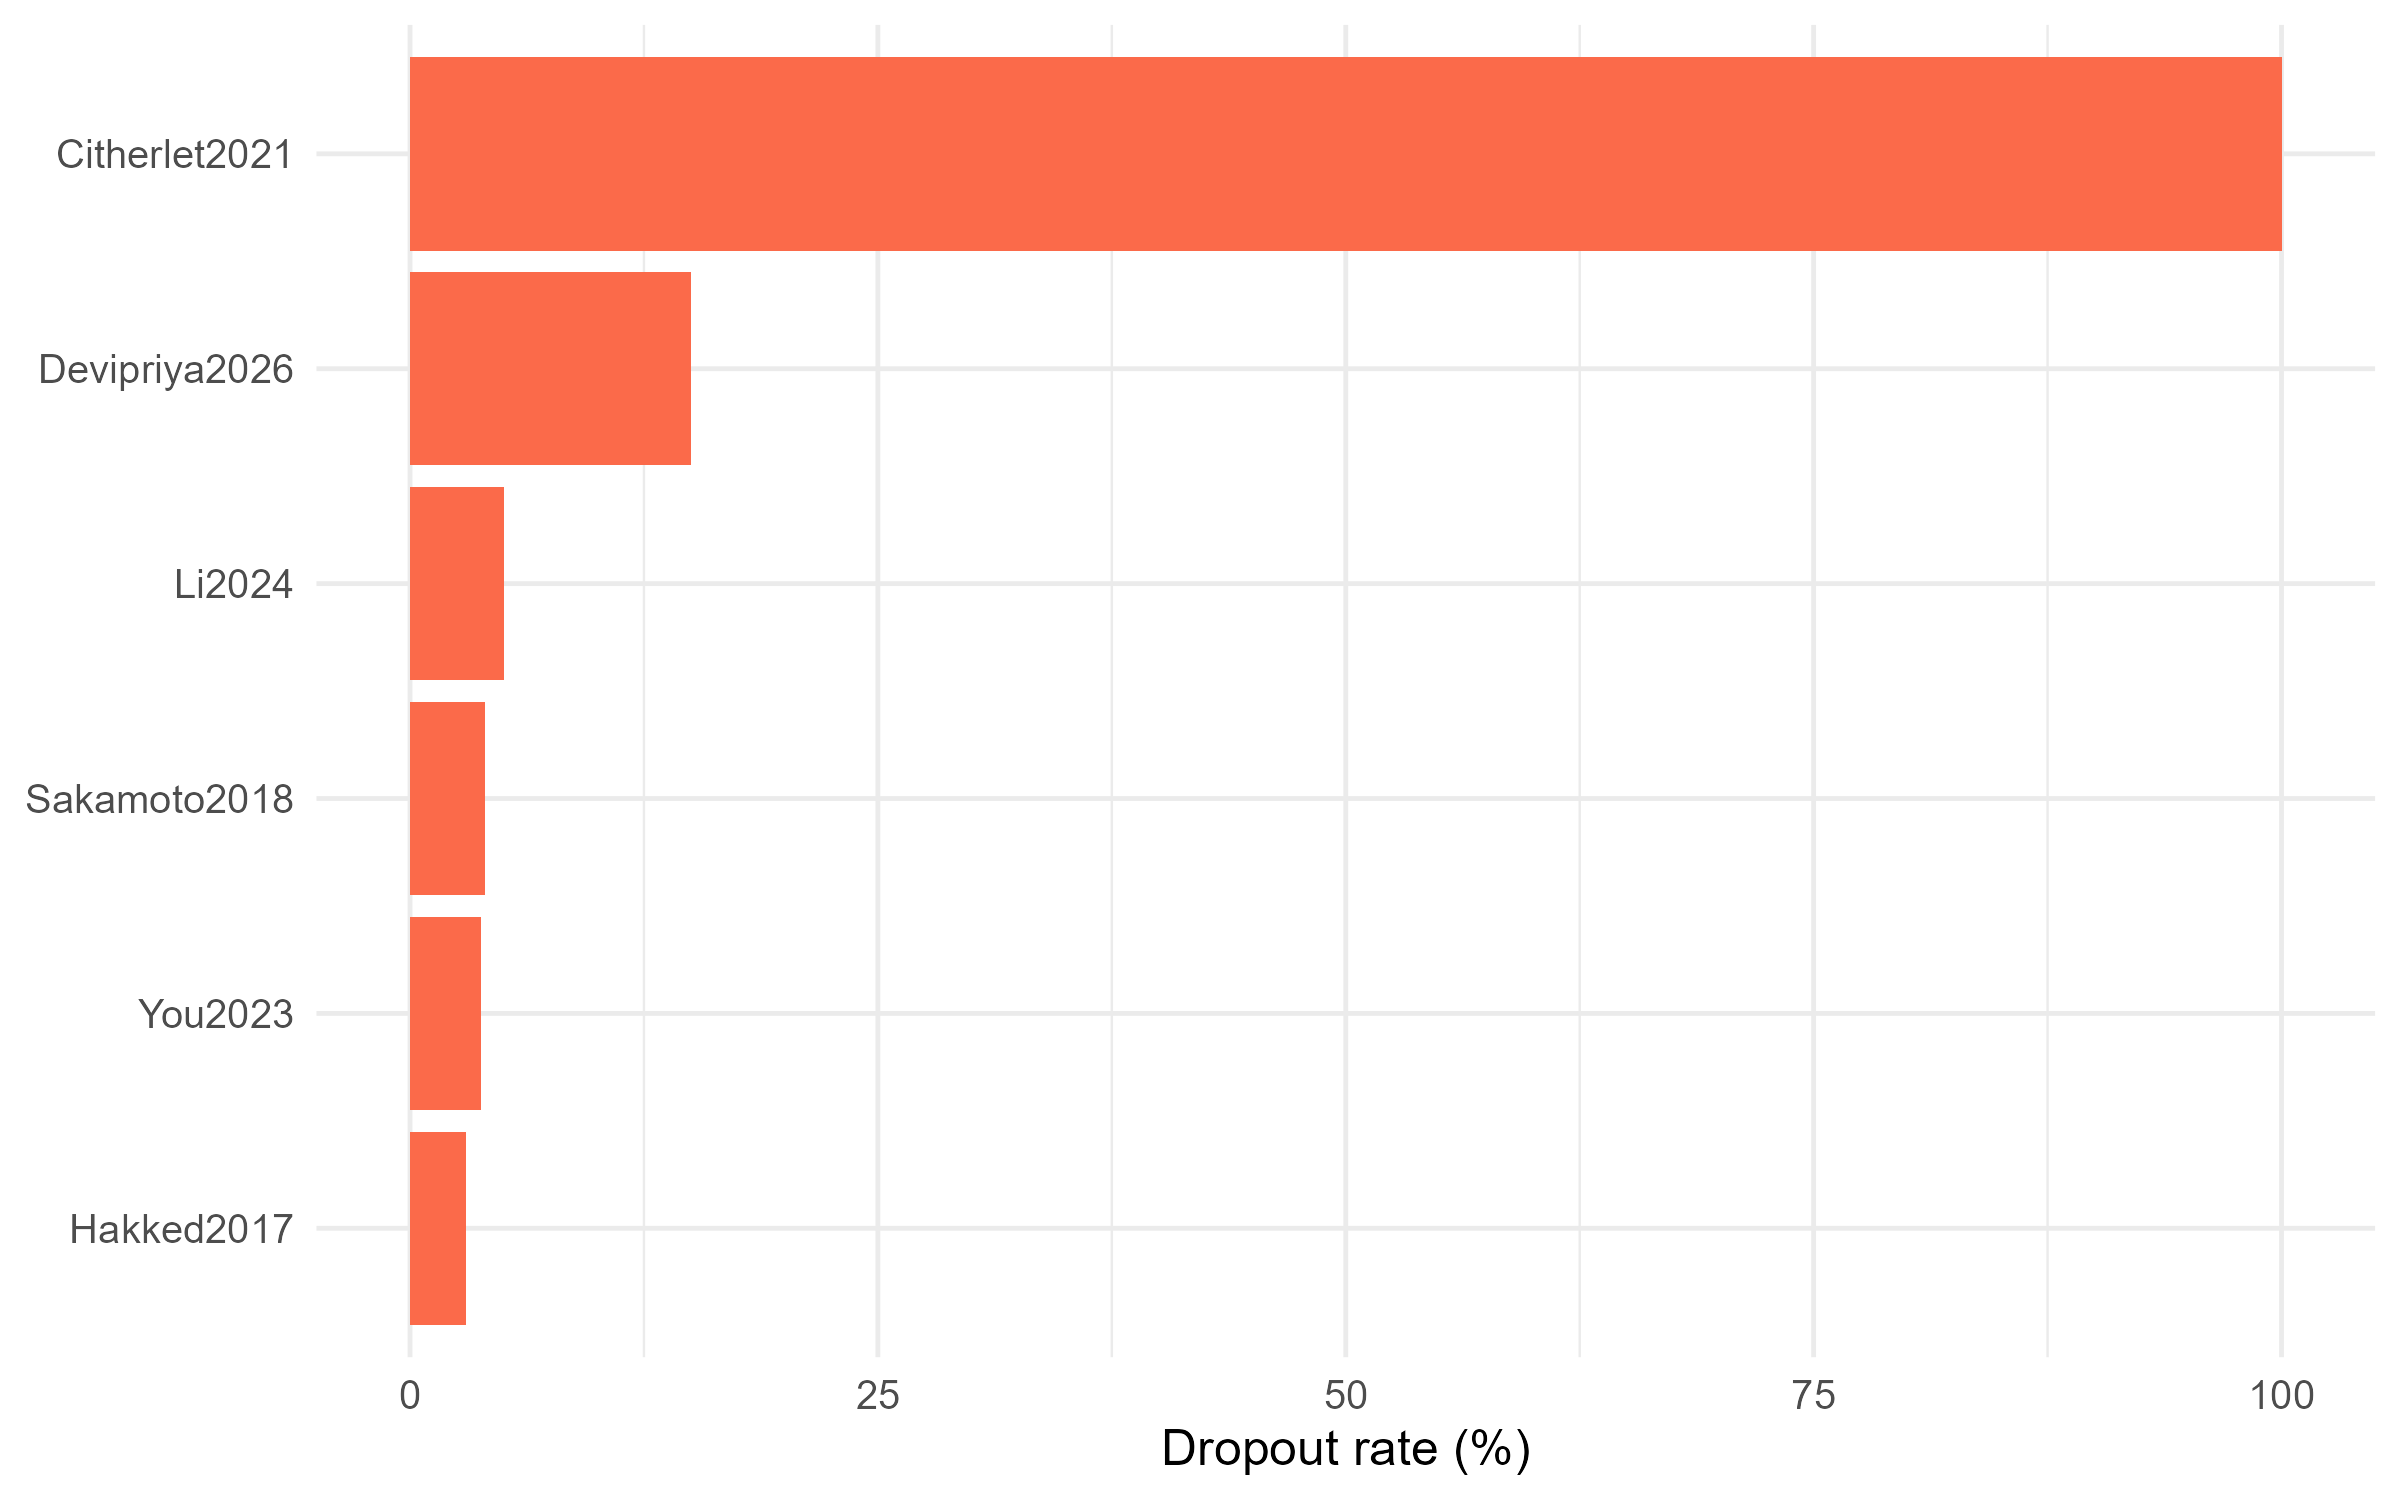
\includegraphics[width=0.82\textwidth]{dropout_rates.png}
\caption{Dropout-rate plot generated from feasibility outputs.}
\label{fig:dropout-rates}
\end{figure}

The dropout plot is included for completeness because it was generated in the analysis outputs, but the cleaned feasibility summary contained no parseable dropout data. The practical interpretation is therefore not that dropout was absent, but that dropout reporting was not extractable in a standardized way from the charted records.

\section{Discussion}
\subsection{Summary of evidence}
This scoping review mapped 34 sources on breathing-training and breath-regulation strategies in sport, exercise, and performance-relevant contexts. The evidence base is broad but fragmented. The included sources span several mechanistically different practices, including hyperventilation, hypoventilation, paced breathing, pranayama/yogic breathing, breath holding, Valsalva-type strategies, hook breathing, and Wim Hof-type breathing. Most studies were experimental, but the dominant pattern was small, acute, crossover, pilot, or repeated-measures work rather than large, preregistered, sport-specific trials.

The most practically relevant finding is not that one breathing method is clearly superior. Rather, the map shows that different breathing strategies are being used for different purposes and should be evaluated separately. Hyperventilation studies tend to target high-intensity power, sprint, blood-gas, or fatigue-related outcomes. Paced breathing is more often directed toward reaction time, recovery, heart-rate variability, stress, or anxiety. Hypoventilation and breath-holding studies are concentrated in repeated-sprint, swimming, judo, freediving, or oxygen-tolerance contexts. Pranayama/yogic studies often examine pulmonary, reaction-time, or broader performance-related outcomes.

The exploratory effect-size summaries are consistent with this interpretation. Hyperventilation showed a small, borderline pooled effect on power-related outcomes, but confidence intervals included a null effect. Paced breathing did not show a clear pooled benefit for reaction outcomes and showed moderate heterogeneity. These analyses are useful for identifying candidate domains for future systematic review, but they are not sufficient for definitive recommendations.

\subsection{Implications for practice}
Practitioners should avoid treating ``breathwork'' as a single intervention class. Acute hyperventilation, slow-paced breathing, hook breathing, hypoventilation, and pranayama differ in physiological targets, risk profile, and likely performance relevance. The mapped evidence suggests that some methods may be promising in narrowly matched contexts, such as hyperventilation before or between high-intensity bouts, paced breathing for psychophysiological regulation, and hypoventilation in repeated-sprint or aquatic contexts. However, practical use should remain conservative because many studies are small, short-term, and incompletely reported.

\subsection{Implications for research}
Future studies should define the breathing intervention precisely, including respiratory rate, depth, timing relative to exercise, session frequency, total exposure, supervision, and safety monitoring. Trials should select outcomes that match the hypothesized mechanism, report adherence and dropout, and preregister analysis plans. Sport-specific studies should distinguish elite, competitive, recreational, and non-athlete populations. The field would also benefit from a shared taxonomy separating ventilatory manipulation, autonomic regulation, respiratory-muscle practice, apnea/hypoventilation exposure, and meditative or yogic breathing practices.

\subsection{Limitations}
This manuscript was generated from the available AIK-SCR extraction and analysis files and from the project documents `paper/docs/introduction.md' and `paper/docs/pubmed-string.md'. The PubMed search string, search date, and initial yield were available, but duplicate-removal details and full-text exclusion reasons were not present in the current project files. Some bibliographic records in `articles.bib' were difficult to reconcile with extraction IDs; Fernandez 2019, Fernandez 2025, and Devipriya 2026 were present in the extraction material but not reliably matched to a BibTeX entry by the available Rayyan export keys. One cleaned row lost the lowercase `bahensky2021' identifier because the cleaning rule expected uppercase AuthorYear formatting. These issues should be reconciled before journal submission.

The effect-size analyses also have limitations. They rely on extracted group means and dispersions treated as standard deviations, combine only small clusters, and normalize effect directions algorithmically. As a result, the quantitative summaries should be interpreted as exploratory signals within a scoping review, not as conclusive evidence of efficacy.

\section{Conclusions}
The AIK-SCR evidence map shows a rapidly developing but heterogeneous literature on breathing strategies in sport and performance settings. The current evidence is strongest as a map of concepts, contexts, and gaps. Hyperventilation may have a small acute signal for power-related outcomes, while paced-breathing effects on reaction outcomes remain uncertain. Feasibility and safety reporting are major weaknesses across the corpus. Publication-ready future work should use clearer taxonomies, complete reporting, and sport-specific, adequately powered comparative designs before strong practical recommendations are made.

\section*{Declarations}
\textbf{Funding:} No funding information was available in the project files.\\
\textbf{Conflicts of interest:} No conflicts of interest were recorded in the project files.\\
\textbf{Data availability:} The extracted data, analysis scripts, generated tables, and figures are available in the AIK-SCR project folders `Data`, `scripts`, and `outputs`.\\
\textbf{Author contributions:} Data extraction, cleaning, analysis, and manuscript drafting should be completed with named contributors before submission.

\appendix
\section{PRISMA-ScR Checklist Crosswalk}
\begin{longtable}{@{}p{0.18\linewidth}p{0.50\linewidth}p{0.22\linewidth}@{}}
\caption{PRISMA-ScR reporting checklist crosswalk for this manuscript.}
\label{tab:prisma-checklist}\\
\toprule
Item & Reporting element & Location in manuscript \\
\midrule
\endfirsthead
\toprule
Item & Reporting element & Location in manuscript \\
\midrule
\endhead
\bottomrule
\endfoot
Title & Identifies the report as a scoping review & Title page \\
Abstract & Structured summary including background, objectives, eligibility, sources, charting, results, conclusions & Abstract \\
Rationale & Rationale for mapping the evidence & Introduction \\
Objectives & Review question and objectives & Introduction \\
Protocol and registration & Protocol status reported & Methods \\
Eligibility criteria & Population, concept, context, source characteristics & Methods \\
Information sources & PubMed and citation backtracking reported & Methods \\
Search & Search source count reported; exact string/date unavailable & Methods; limitations \\
Selection of sources & Screening stages and counts reported & Methods; Figure~\ref{fig:prisma} \\
Data charting process & Extraction, cleaning, and charting variables reported & Methods \\
Data items & Bibliometric, demographic, intervention, outcome, feasibility, and safety variables reported & Methods \\
Critical appraisal & Not performed as a formal quality appraisal; data completeness appraised descriptively & Methods; limitations \\
Synthesis & Narrative mapping plus exploratory effect-size summaries & Methods; Results \\
Selection results & Counts at each screening stage & Results; Figure~\ref{fig:prisma} \\
Characteristics & Included-source characteristics & Results; Table~\ref{tab:study-characteristics} \\
Critical appraisal results & Data-quality issues summarized where relevant & Results; limitations \\
Individual-source results & Study-level characteristics and outcome clusters summarized & Results; appendices \\
Synthesis of results & Evidence map, plots, tables, and exploratory syntheses & Results \\
Summary of evidence & Main findings linked to objectives & Discussion \\
Limitations & Review and evidence-base limitations & Discussion \\
Conclusions & Interpretation and next steps & Conclusions \\
Funding & Funding statement placeholder included & Declarations \\
\end{longtable}


\section{Referenced Included Sources}
\nocite{rayyan-164849052,rayyan-164849040,rayyan-164849036,rayyan-164848982,rayyan-164849000,rayyan-164848980,rayyan-164848972,rayyan-164848960,rayyan-164848964,rayyan-164848918,rayyan-587891674,rayyan-164848916,rayyan-164848919,rayyan-164848909,rayyan-164848882,rayyan-164848876,rayyan-164848862,rayyan-164848878,rayyan-164848880,rayyan-164848859,rayyan-587869979,rayyan-587870003,rayyan-587869980,rayyan-587869976,rayyan-587869968,rayyan-587869999,rayyan-587870002,rayyan-587870000,rayyan-587870001,rayyan-587869988,rayyan-587869986}
\printbibliography

\end{document}
